% Supplementary material. Built with: make supplement (from paper/).
\documentclass[11pt]{article}
\usepackage[margin=2.2cm]{geometry}
\usepackage[T1]{fontenc}
\usepackage{lmodern}
\usepackage{microtype}
\usepackage{xspace}
\usepackage{amsmath}
\usepackage{booktabs}
\usepackage{array}
\usepackage[section]{placeins}
\usepackage{longtable}
\usepackage{graphicx}
\usepackage[numbers,sort&compress]{natbib}
\usepackage[hidelinks]{hyperref}
\usepackage{xcolor}
\usepackage{tikz}
\usetikzlibrary{positioning,arrows.meta}
\definecolor{ink}{HTML}{0B0B0B}
\definecolor{ink2}{HTML}{52514E}
\definecolor{auditfill}{HTML}{FCEDE6}
\definecolor{gemfill}{HTML}{E9F1FB}
\graphicspath{{figures/}}
% Generated by paper/scripts/make_numbers.py. Do not edit by hand.
\newcommand{\NGenomes}{754\xspace}
\newcommand{\NSpecies}{669\xspace}
\newcommand{\NSlow}{58\xspace}
\newcommand{\NArchaea}{156\xspace}
\newcommand{\NInputs}{56\xspace}
\newcommand{\NLiterature}{8\xspace}
\newcommand{\NGenomeExtension}{161\xspace}
\newcommand{\NOriginal}{294\xspace}
\newcommand{\NMadinExtension}{291\xspace}
\newcommand{\NExcluded}{10\xspace}
\newcommand{\NExcludedKevbrina}{4\xspace}
\newcommand{\NExcludedWord}{ten\xspace}
\newcommand{\NExcludedKevbrinaWord}{four\xspace}
\newcommand{\NExcludedSourcesWord}{five\xspace}
\newcommand{\NLiteratureWord}{eight\xspace}
\newcommand{\ErrSameGenus}{1.75\xspace}
\newcommand{\RhoSameGenus}{0.74\xspace}
\newcommand{\AucSameGenus}{0.85\xspace}
\newcommand{\ErrRefSameGenus}{1.73\xspace}
\newcommand{\RhoRefSameGenus}{0.84\xspace}
\newcommand{\TempMAESameGenus}{5.0\xspace}
\newcommand{\RhoTempSameGenus}{0.86\xspace}
\newcommand{\FixedErrSameGenus}{1.82\xspace}
\newcommand{\CoarseErrSameGenus}{1.75\xspace}
\newcommand{\FixedErrRefSameGenus}{1.75\xspace}
\newcommand{\ErrNewGenus}{1.91\xspace}
\newcommand{\RhoNewGenus}{0.71\xspace}
\newcommand{\AucNewGenus}{0.84\xspace}
\newcommand{\ErrRefNewGenus}{1.81\xspace}
\newcommand{\RhoRefNewGenus}{0.83\xspace}
\newcommand{\TempMAENewGenus}{5.7\xspace}
\newcommand{\RhoTempNewGenus}{0.83\xspace}
\newcommand{\FixedErrNewGenus}{1.96\xspace}
\newcommand{\CoarseErrNewGenus}{1.92\xspace}
\newcommand{\FixedErrRefNewGenus}{1.79\xspace}
\newcommand{\ErrNewFamily}{2.06\xspace}
\newcommand{\RhoNewFamily}{0.66\xspace}
\newcommand{\AucNewFamily}{0.81\xspace}
\newcommand{\ErrRefNewFamily}{1.91\xspace}
\newcommand{\RhoRefNewFamily}{0.81\xspace}
\newcommand{\TempMAENewFamily}{5.8\xspace}
\newcommand{\RhoTempNewFamily}{0.83\xspace}
\newcommand{\FixedErrNewFamily}{2.07\xspace}
\newcommand{\CoarseErrNewFamily}{2.07\xspace}
\newcommand{\FixedErrRefNewFamily}{1.88\xspace}
\newcommand{\ErrNewOrder}{2.08\xspace}
\newcommand{\RhoNewOrder}{0.66\xspace}
\newcommand{\AucNewOrder}{0.82\xspace}
\newcommand{\ErrRefNewOrder}{1.93\xspace}
\newcommand{\RhoRefNewOrder}{0.81\xspace}
\newcommand{\TempMAENewOrder}{6.0\xspace}
\newcommand{\RhoTempNewOrder}{0.81\xspace}
\newcommand{\FixedErrNewOrder}{2.08\xspace}
\newcommand{\CoarseErrNewOrder}{2.08\xspace}
\newcommand{\FixedErrRefNewOrder}{1.91\xspace}
\newcommand{\NSeedsHeadline}{3\xspace}
\newcommand{\NHeadlineRows}{742\xspace}
\newcommand{\SlowCalledSpecies}{9\xspace}
\newcommand{\SlowCalledTrueSpecies}{8\xspace}
\newcommand{\SlowTotalSpecies}{52\xspace}
\newcommand{\SlowCalledOrder}{0\xspace}
\newcommand{\SlowCalledTrueOrder}{0\xspace}
\newcommand{\SlowTotalOrder}{52\xspace}
\newcommand{\CoverSameGenus}{80\xspace}
\newcommand{\CoverNewGenus}{80\xspace}
\newcommand{\CoverNewFamily}{80\xspace}
\newcommand{\CoverNewOrder}{81\xspace}
\newcommand{\CoverRefMin}{79\xspace}
\newcommand{\CoverRefMax}{80\xspace}
\newcommand{\CoverTempMin}{81\xspace}
\newcommand{\CoverTempMax}{84\xspace}
\newcommand{\NGEMPredicted}{9,139\xspace}
\newcommand{\GEMShareSameGenus}{11\xspace}
\newcommand{\GEMShareNewGenus}{24\xspace}
\newcommand{\GEMShareNewFamily}{27\xspace}
\newcommand{\GEMShareNewOrder}{38\xspace}
\newcommand{\GEMShareNoGenus}{89\xspace}
\newcommand{\GEMMedianHours}{2.8\xspace}
\newcommand{\GEMShareSlow}{0.4\xspace}
\newcommand{\GEMNSlow}{39\xspace}
\newcommand{\GEMSlowTopOrder}{Anaerolineales\xspace}
\newcommand{\GEMSlowTopOrderN}{21\xspace}
\newcommand{\GEMMedianHuman}{1.6\xspace}
\newcommand{\GEMNHuman}{3,747\xspace}
\newcommand{\GEMNewOrderHuman}{26\xspace}
\newcommand{\GEMMedianAquatic}{6.7\xspace}
\newcommand{\GEMNAquatic}{2,522\xspace}
\newcommand{\GEMNewOrderAquatic}{58\xspace}
\newcommand{\GEMMedianBuilt}{1.0\xspace}
\newcommand{\GEMNBuilt}{915\xspace}
\newcommand{\GEMNewOrderBuilt}{10\xspace}
\newcommand{\GEMMedianTerrestrial}{7.3\xspace}
\newcommand{\GEMNTerrestrial}{497\xspace}
\newcommand{\GEMNewOrderTerrestrial}{55\xspace}
\newcommand{\GEMMedianWastewater}{7.1\xspace}
\newcommand{\GEMNWastewater}{492\xspace}
\newcommand{\GEMNewOrderWastewater}{60\xspace}
\newcommand{\GEMSlowSecondOrder}{Nitrososphaerales\xspace}
\newcommand{\GEMSlowSecondOrderN}{13\xspace}
\newcommand{\RelOursErr}{1.76\xspace}
\newcommand{\RelOursRho}{0.72\xspace}
\newcommand{\RelOursAuc}{0.85\xspace}
\newcommand{\RelOursTempErr}{1.70\xspace}
\newcommand{\RelOursTempRho}{0.76\xspace}
\newcommand{\RelOursTempAuc}{0.87\xspace}
\newcommand{\RelGRodonErr}{1.92\xspace}
\newcommand{\RelGRodonRho}{0.73\xspace}
\newcommand{\RelGRodonAuc}{0.84\xspace}
\newcommand{\RelGRodonNoTempErr}{2.40\xspace}
\newcommand{\RelGRodonNoTempRho}{0.52\xspace}
\newcommand{\RelGRodonNoTempAuc}{0.75\xspace}
\newcommand{\RelPhydonErr}{1.85\xspace}
\newcommand{\RelPhydonRho}{0.70\xspace}
\newcommand{\RelPhydonAuc}{0.81\xspace}
\newcommand{\RelN}{680\xspace}
\newcommand{\RelNPhydon}{665\xspace}
\newcommand{\RelNSeeds}{3\xspace}
\newcommand{\RelOursTempBeatsPhydon}{3\xspace}
\newcommand{\RelOursTempBeatsGRodon}{3\xspace}
\newcommand{\RelOursBeatsPhydon}{3\xspace}
\newcommand{\RelOursBeatsGRodon}{3\xspace}
\newcommand{\PosCtrlCaughtWord}{eight\xspace}
\newcommand{\PosCtrlNWord}{nine\xspace}
\newcommand{\KevFoldWith}{5.2\xspace}
\newcommand{\KevLowWith}{2.1\xspace}
\newcommand{\KevHighWith}{12.7\xspace}
\newcommand{\KevPWith}{0.01\xspace}
\newcommand{\KevNWith}{11\xspace}
\newcommand{\KevFoldWithout}{1.5\xspace}
\newcommand{\KevLowWithout}{0.5\xspace}
\newcommand{\KevHighWithout}{4.8\xspace}
\newcommand{\KevPWithout}{0.90\xspace}
\newcommand{\KevNWithout}{7\xspace}
\newcommand{\KevLabelMin}{112\xspace}
\newcommand{\KevLabelMax}{187\xspace}
\newcommand{\KevRecordMin}{2,717\xspace}
\newcommand{\KevRecordMax}{4,576\xspace}
\newcommand{\KevRatio}{24\xspace}
\newcommand{\NStudiesCompared}{27\xspace}
\newcommand{\NStudiesFlagged}{8\xspace}
\newcommand{\SixteenOwnDist}{0.036\xspace}
\newcommand{\SixteenNearDist}{0.158\xspace}
\newcommand{\SixteenN}{540\xspace}
\newcommand{\SixteenFarther}{65\xspace}
\newcommand{\SixteenShift}{0.09\xspace}
\newcommand{\SixteenNGenomeCopy}{685\xspace}
\newcommand{\SixteenErrNcbiSpecies}{1.76\xspace}
\newcommand{\SixteenErrGenomeSpecies}{1.75\xspace}
\newcommand{\SixteenErrMixedSpecies}{1.79\xspace}
\newcommand{\SixteenMixedWorseSpecies}{3\xspace}
\newcommand{\SixteenErrNcbiOrder}{1.98\xspace}
\newcommand{\SixteenErrGenomeOrder}{1.97\xspace}
\newcommand{\SixteenErrMixedOrder}{2.03\xspace}
\newcommand{\SixteenMixedWorseOrder}{3\xspace}
\newcommand{\SixteenNSeeds}{3\xspace}
\newcommand{\NSeedsAblation}{10\xspace}
\newcommand{\AblFinalErrSpecies}{1.82\xspace}
\newcommand{\AblFinalRhoSpecies}{0.74\xspace}
\newcommand{\AblFinalAucSpecies}{0.84\xspace}
\newcommand{\AblGStatErrSpecies}{1.93\xspace}
\newcommand{\AblGStatRhoSpecies}{0.70\xspace}
\newcommand{\AblGStatAucSpecies}{0.83\xspace}
\newcommand{\AblGStatWorseSpecies}{10\xspace}
\newcommand{\AblLifeErrSpecies}{1.82\xspace}
\newcommand{\AblLifeRhoSpecies}{0.74\xspace}
\newcommand{\AblLifeAucSpecies}{0.84\xspace}
\newcommand{\AblLifeWorseSpecies}{6\xspace}
\newcommand{\AblGenesErrSpecies}{2.09\xspace}
\newcommand{\AblGenesRhoSpecies}{0.66\xspace}
\newcommand{\AblGenesAucSpecies}{0.81\xspace}
\newcommand{\AblGenesWorseSpecies}{10\xspace}
\newcommand{\AblSixteenErrSpecies}{1.82\xspace}
\newcommand{\AblSixteenRhoSpecies}{0.74\xspace}
\newcommand{\AblSixteenAucSpecies}{0.84\xspace}
\newcommand{\AblSixteenWorseSpecies}{3\xspace}
\newcommand{\AblPhyloErrSpecies}{1.84\xspace}
\newcommand{\AblPhyloRhoSpecies}{0.73\xspace}
\newcommand{\AblPhyloAucSpecies}{0.84\xspace}
\newcommand{\AblPhyloWorseSpecies}{9\xspace}
\newcommand{\AblAddedErrSpecies}{1.86\xspace}
\newcommand{\AblAddedRhoSpecies}{0.73\xspace}
\newcommand{\AblAddedAucSpecies}{0.84\xspace}
\newcommand{\AblAddedWorseSpecies}{10\xspace}
\newcommand{\AblEnergyErrSpecies}{1.82\xspace}
\newcommand{\AblEnergyRhoSpecies}{0.74\xspace}
\newcommand{\AblEnergyAucSpecies}{0.84\xspace}
\newcommand{\AblEnergyWorseSpecies}{6\xspace}
\newcommand{\AblPredTempErrSpecies}{1.80\xspace}
\newcommand{\AblPredTempRhoSpecies}{0.74\xspace}
\newcommand{\AblPredTempAucSpecies}{0.84\xspace}
\newcommand{\AblPredTempWorseSpecies}{4\xspace}
\newcommand{\AblFinalErrOrder}{2.09\xspace}
\newcommand{\AblFinalRhoOrder}{0.65\xspace}
\newcommand{\AblFinalAucOrder}{0.80\xspace}
\newcommand{\AblGStatErrOrder}{2.39\xspace}
\newcommand{\AblGStatRhoOrder}{0.57\xspace}
\newcommand{\AblGStatAucOrder}{0.76\xspace}
\newcommand{\AblGStatWorseOrder}{10\xspace}
\newcommand{\AblLifeErrOrder}{2.07\xspace}
\newcommand{\AblLifeRhoOrder}{0.66\xspace}
\newcommand{\AblLifeAucOrder}{0.81\xspace}
\newcommand{\AblLifeWorseOrder}{4\xspace}
\newcommand{\AblGenesErrOrder}{2.64\xspace}
\newcommand{\AblGenesRhoOrder}{0.46\xspace}
\newcommand{\AblGenesAucOrder}{0.73\xspace}
\newcommand{\AblGenesWorseOrder}{10\xspace}
\newcommand{\AblSixteenErrOrder}{2.09\xspace}
\newcommand{\AblSixteenRhoOrder}{0.65\xspace}
\newcommand{\AblSixteenAucOrder}{0.79\xspace}
\newcommand{\AblSixteenWorseOrder}{4\xspace}
\newcommand{\AblPhyloErrOrder}{2.07\xspace}
\newcommand{\AblPhyloRhoOrder}{0.66\xspace}
\newcommand{\AblPhyloAucOrder}{0.81\xspace}
\newcommand{\AblPhyloWorseOrder}{2\xspace}
\newcommand{\AblAddedErrOrder}{2.13\xspace}
\newcommand{\AblAddedRhoOrder}{0.65\xspace}
\newcommand{\AblAddedAucOrder}{0.80\xspace}
\newcommand{\AblAddedWorseOrder}{10\xspace}
\newcommand{\AblEnergyErrOrder}{2.11\xspace}
\newcommand{\AblEnergyRhoOrder}{0.65\xspace}
\newcommand{\AblEnergyAucOrder}{0.80\xspace}
\newcommand{\AblEnergyWorseOrder}{7\xspace}
\newcommand{\AblPredTempErrOrder}{2.08\xspace}
\newcommand{\AblPredTempRhoOrder}{0.66\xspace}
\newcommand{\AblPredTempAucOrder}{0.80\xspace}
\newcommand{\AblPredTempWorseOrder}{2\xspace}
\newcommand{\TuneErrBefore}{2.14\xspace}
\newcommand{\TuneErrAfter}{2.13\xspace}
\newcommand{\TuneRhoBefore}{0.63\xspace}
\newcommand{\TuneRhoAfter}{0.65\xspace}
\newcommand{\TuneAucBefore}{0.79\xspace}
\newcommand{\TuneAucAfter}{0.80\xspace}
\newcommand{\TuneBetter}{4\xspace}
\newcommand{\TuneNSeeds}{5\xspace}
\newcommand{\MagErr}{1.86\xspace}
\newcommand{\MagIsoErr}{1.70\xspace}
\newcommand{\MagNSpecies}{47\xspace}
\newcommand{\MagNGenomes}{717\xspace}
\newcommand{\MagGap}{1.08\xspace}
\newcommand{\MagGapMax}{2.2\xspace}
\newcommand{\MagGapSmaller}{41\xspace}
\newcommand{\IndepErr}{2.09\xspace}
\newcommand{\IndepN}{294\xspace}
\newcommand{\BaseRelErrSameGenus}{1.81\xspace}
\newcommand{\BaseRelRhoSameGenus}{0.66\xspace}
\newcommand{\BaseRelAucSameGenus}{0.80\xspace}
\newcommand{\BaseMedErrSameGenus}{2.72\xspace}
\newcommand{\CIErrLoSameGenus}{1.67\xspace}
\newcommand{\CIErrHiSameGenus}{1.86\xspace}
\newcommand{\CIRhoLoSameGenus}{0.68\xspace}
\newcommand{\CIRhoHiSameGenus}{0.78\xspace}
\newcommand{\CIDiffLoSameGenus}{$-$0.21\xspace}
\newcommand{\CIDiffHiSameGenus}{0.05\xspace}
\newcommand{\BaseRelErrNewGenus}{2.12\xspace}
\newcommand{\BaseRelRhoNewGenus}{0.57\xspace}
\newcommand{\BaseRelAucNewGenus}{0.79\xspace}
\newcommand{\BaseMedErrNewGenus}{2.74\xspace}
\newcommand{\CIErrLoNewGenus}{1.81\xspace}
\newcommand{\CIErrHiNewGenus}{2.02\xspace}
\newcommand{\CIRhoLoNewGenus}{0.66\xspace}
\newcommand{\CIRhoHiNewGenus}{0.76\xspace}
\newcommand{\CIDiffLoNewGenus}{$-$0.42\xspace}
\newcommand{\CIDiffHiNewGenus}{$-$0.02\xspace}
\newcommand{\BaseRelErrNewFamily}{2.59\xspace}
\newcommand{\BaseRelRhoNewFamily}{0.40\xspace}
\newcommand{\BaseRelAucNewFamily}{0.72\xspace}
\newcommand{\BaseMedErrNewFamily}{2.86\xspace}
\newcommand{\CIErrLoNewFamily}{1.93\xspace}
\newcommand{\CIErrHiNewFamily}{2.24\xspace}
\newcommand{\CIRhoLoNewFamily}{0.59\xspace}
\newcommand{\CIRhoHiNewFamily}{0.72\xspace}
\newcommand{\CIDiffLoNewFamily}{$-$0.84\xspace}
\newcommand{\CIDiffHiNewFamily}{$-$0.21\xspace}
\newcommand{\BaseRelErrNewOrder}{2.45\xspace}
\newcommand{\BaseRelRhoNewOrder}{0.41\xspace}
\newcommand{\BaseRelAucNewOrder}{0.72\xspace}
\newcommand{\BaseMedErrNewOrder}{2.78\xspace}
\newcommand{\CIErrLoNewOrder}{1.96\xspace}
\newcommand{\CIErrHiNewOrder}{2.23\xspace}
\newcommand{\CIRhoLoNewOrder}{0.57\xspace}
\newcommand{\CIRhoHiNewOrder}{0.72\xspace}
\newcommand{\CIDiffLoNewOrder}{$-$0.74\xspace}
\newcommand{\CIDiffHiNewOrder}{$-$0.16\xspace}
\newcommand{\ShuffleErrSpecies}{2.91\xspace}
\newcommand{\ShuffleRhoSpecies}{0.00\xspace}
\newcommand{\ShuffleMedErrSpecies}{2.73\xspace}
\newcommand{\ShuffleErrOrder}{2.89\xspace}
\newcommand{\ShuffleRhoOrder}{$-$0.04\xspace}
\newcommand{\ShuffleMedErrOrder}{2.72\xspace}
\newcommand{\PairGRodonN}{680\xspace}
\newcommand{\PairGRodonBetter}{349\xspace}
\newcommand{\PairGRodonP}{0.07\xspace}
\newcommand{\PairGRodonDiffLo}{$-$0.26\xspace}
\newcommand{\PairGRodonDiffHi}{$-$0.04\xspace}
\newcommand{\PairTempGRodonN}{680\xspace}
\newcommand{\PairTempGRodonBetter}{383\xspace}
\newcommand{\PairTempGRodonP}{$1.5\times10^{-6}$\xspace}
\newcommand{\PairPhydonN}{665\xspace}
\newcommand{\PairPhydonBetter}{347\xspace}
\newcommand{\PairPhydonP}{0.11\xspace}
\newcommand{\PairPhydonDiffLo}{$-$0.26\xspace}
\newcommand{\PairPhydonDiffHi}{0.05\xspace}
\newcommand{\PairTempPhydonN}{665\xspace}
\newcommand{\PairTempPhydonBetter}{355\xspace}
\newcommand{\PairTempPhydonP}{$3.9\times10^{-4}$\xspace}
\newcommand{\CIMagErrLo}{1.60\xspace}
\newcommand{\CIMagErrHi}{2.20\xspace}
\newcommand{\CIMagDiffLo}{$-$0.16\xspace}
\newcommand{\CIMagDiffHi}{0.32\xspace}
\newcommand{\CovNovAllSpecies}{80\xspace}
\newcommand{\CovNovArchSpecies}{79\xspace}
\newcommand{\CovNovSlowSpecies}{44\xspace}
\newcommand{\CovNovFastSpecies}{83\xspace}
\newcommand{\CovDomAllSpecies}{80\xspace}
\newcommand{\CovDomArchSpecies}{79\xspace}
\newcommand{\CovDomSlowSpecies}{45\xspace}
\newcommand{\CovDomFastSpecies}{83\xspace}
\newcommand{\CovNovAllOrder}{80\xspace}
\newcommand{\CovNovArchOrder}{73\xspace}
\newcommand{\CovNovSlowOrder}{26\xspace}
\newcommand{\CovNovFastOrder}{85\xspace}
\newcommand{\CovDomAllOrder}{79\xspace}
\newcommand{\CovDomArchOrder}{78\xspace}
\newcommand{\CovDomSlowOrder}{29\xspace}
\newcommand{\CovDomFastOrder}{83\xspace}
\newcommand{\CovDomArchMin}{78\xspace}
\newcommand{\CovDomSlowMin}{29\xspace}
\newcommand{\CovDomSlowMax}{45\xspace}
\newcommand{\SlowProbAucSpecies}{0.84\xspace}
\newcommand{\SlowProbTopSpecies}{24\xspace}
\newcommand{\SlowProbBrierSpecies}{0.057\xspace}
\newcommand{\SlowProbBrierBaseSpecies}{0.072\xspace}
\newcommand{\SlowProbAucOrder}{0.81\xspace}
\newcommand{\SlowProbTopOrder}{22\xspace}
\newcommand{\SlowProbBrierOrder}{0.065\xspace}
\newcommand{\SlowProbBrierBaseOrder}{0.072\xspace}
\newcommand{\SlowProbECEMax}{0.012\xspace}
\newcommand{\SlowBaseRate}{8\xspace}
\newcommand{\ErrSlowSpecies}{4.5\xspace}
\newcommand{\ErrArchSpecies}{1.87\xspace}
\newcommand{\ErrBactSpecies}{1.72\xspace}
\newcommand{\ErrSlowOrder}{6.3\xspace}
\newcommand{\ErrArchOrder}{2.43\xspace}
\newcommand{\ErrBactOrder}{2.02\xspace}
\newcommand{\GEMNArchaea}{183\xspace}
\newcommand{\EsmN}{742\xspace}
\newcommand{\EsmFeatErrSameGenus}{1.82\xspace}
\newcommand{\EsmFeatRhoSameGenus}{0.74\xspace}
\newcommand{\EsmProbeErrSameGenus}{1.86\xspace}
\newcommand{\EsmProbeRhoSameGenus}{0.75\xspace}
\newcommand{\EsmTreesErrSameGenus}{2.03\xspace}
\newcommand{\EsmTreesRhoSameGenus}{0.71\xspace}
\newcommand{\EsmCombErrSameGenus}{1.78\xspace}
\newcommand{\EsmCombRhoSameGenus}{0.76\xspace}
\newcommand{\EsmFeatErrNewGenus}{1.96\xspace}
\newcommand{\EsmFeatRhoNewGenus}{0.71\xspace}
\newcommand{\EsmProbeErrNewGenus}{1.90\xspace}
\newcommand{\EsmProbeRhoNewGenus}{0.73\xspace}
\newcommand{\EsmTreesErrNewGenus}{2.11\xspace}
\newcommand{\EsmTreesRhoNewGenus}{0.67\xspace}
\newcommand{\EsmCombErrNewGenus}{1.91\xspace}
\newcommand{\EsmCombRhoNewGenus}{0.74\xspace}
\newcommand{\EsmFeatErrNewFamily}{2.07\xspace}
\newcommand{\EsmFeatRhoNewFamily}{0.67\xspace}
\newcommand{\EsmProbeErrNewFamily}{2.00\xspace}
\newcommand{\EsmProbeRhoNewFamily}{0.69\xspace}
\newcommand{\EsmTreesErrNewFamily}{2.19\xspace}
\newcommand{\EsmTreesRhoNewFamily}{0.62\xspace}
\newcommand{\EsmCombErrNewFamily}{2.03\xspace}
\newcommand{\EsmCombRhoNewFamily}{0.70\xspace}
\newcommand{\EsmFeatErrNewOrder}{2.08\xspace}
\newcommand{\EsmFeatRhoNewOrder}{0.67\xspace}
\newcommand{\EsmProbeErrNewOrder}{2.02\xspace}
\newcommand{\EsmProbeRhoNewOrder}{0.68\xspace}
\newcommand{\EsmTreesErrNewOrder}{2.23\xspace}
\newcommand{\EsmTreesRhoNewOrder}{0.61\xspace}
\newcommand{\EsmCombErrNewOrder}{2.05\xspace}
\newcommand{\EsmCombRhoNewOrder}{0.70\xspace}
\newcommand{\EsmProbePSameGenus}{0.87\xspace}
\newcommand{\EsmProbeBetterSameGenus}{368\xspace}
\newcommand{\EsmCombPSameGenus}{$3.1\times10^{-4}$\xspace}
\newcommand{\EsmCombBetterSameGenus}{426\xspace}
\newcommand{\EsmPairNSameGenus}{741\xspace}
\newcommand{\EsmProbePNewOrder}{0.99\xspace}
\newcommand{\EsmProbeBetterNewOrder}{357\xspace}
\newcommand{\EsmCombPNewOrder}{$6.1\times10^{-5}$\xspace}
\newcommand{\EsmCombBetterNewOrder}{423\xspace}
\newcommand{\EsmPairNNewOrder}{741\xspace}
\newcommand{\TenNSeeds}{10\xspace}
\newcommand{\TenModelErrSpecies}{1.82\xspace}
\newcommand{\TenBaseErrSpecies}{1.79\xspace}
\newcommand{\TenModelRhoSpecies}{0.74\xspace}
\newcommand{\TenBaseRhoSpecies}{0.67\xspace}
\newcommand{\TenModelWinsSpecies}{3\xspace}
\newcommand{\TenPGenomeSpecies}{0.02\xspace}
\newcommand{\TenModelWinsDeepMin}{10\xspace}
\newcommand{\TenPGenomeDeepMax}{$<$\,10$^{-4}$\xspace}
\newcommand{\RefitErrSpecies}{1.85\xspace}
\newcommand{\RefitFullErrSpecies}{1.82\xspace}
\newcommand{\FlagErrSpecies}{1.79\xspace}
\newcommand{\FlagFullErrSpecies}{1.81\xspace}
\newcommand{\RefitErrOrder}{2.10\xspace}
\newcommand{\RefitFullErrOrder}{2.08\xspace}
\newcommand{\FlagErrOrder}{2.02\xspace}
\newcommand{\FlagFullErrOrder}{2.05\xspace}
\newcommand{\RefitMaxDiff}{0.03\xspace}
\newcommand{\FlagNLabels}{25\xspace}
\newcommand{\DupMaxChange}{0.005\xspace}
\newcommand{\RelOrdOursErr}{2.08\xspace}
\newcommand{\RelOrdOursRho}{0.64\xspace}
\newcommand{\RelOrdOursAuc}{0.82\xspace}
\newcommand{\RelOrdOursTempErr}{1.96\xspace}
\newcommand{\RelOrdOursTempRho}{0.70\xspace}
\newcommand{\RelOrdOursTempAuc}{0.83\xspace}
\newcommand{\RelOrdGRodonErr}{1.92\xspace}
\newcommand{\RelOrdGRodonRho}{0.73\xspace}
\newcommand{\RelOrdGRodonAuc}{0.84\xspace}
\newcommand{\RelOrdGRodonNoTempErr}{2.40\xspace}
\newcommand{\RelOrdGRodonNoTempRho}{0.52\xspace}
\newcommand{\RelOrdGRodonNoTempAuc}{0.75\xspace}
\newcommand{\RelOrdPhydonErr}{2.84\xspace}
\newcommand{\RelOrdPhydonRho}{0.58\xspace}
\newcommand{\RelOrdPhydonAuc}{0.76\xspace}
\newcommand{\PairOrdGRodonN}{680\xspace}
\newcommand{\PairOrdGRodonBetter}{330\xspace}
\newcommand{\PairOrdGRodonP}{0.007\xspace}
\newcommand{\PairOrdPhydonN}{665\xspace}
\newcommand{\PairOrdPhydonBetter}{433\xspace}
\newcommand{\PairOrdPhydonP}{$<$\,10$^{-4}$\xspace}
\newcommand{\PairOrdGRodonNoTempN}{680\xspace}
\newcommand{\PairOrdGRodonNoTempBetter}{406\xspace}
\newcommand{\PairOrdGRodonNoTempP}{$<$\,10$^{-4}$\xspace}
\newcommand{\PairOrdTempGRodonN}{680\xspace}
\newcommand{\PairOrdTempGRodonBetter}{351\xspace}
\newcommand{\PairOrdTempGRodonP}{0.96\xspace}
\newcommand{\ExtNCurated}{51\xspace}
\newcommand{\NSeedsExternal}{5\xspace}
\newcommand{\PhydonOrderMapped}{99.6\xspace}
\newcommand{\ExtNSources}{51\xspace}
\newcommand{\ExtN}{48\xspace}
\newcommand{\ExtNSlow}{7\xspace}
\newcommand{\ExtNArchaea}{3\xspace}
\newcommand{\ExtNSameGenus}{7\xspace}
\newcommand{\ExtNNewGenus}{18\xspace}
\newcommand{\ExtNNewFamily}{9\xspace}
\newcommand{\ExtNNewOrder}{14\xspace}
\newcommand{\ExtModelErr}{2.53\xspace}
\newcommand{\ExtModelLo}{1.91\xspace}
\newcommand{\ExtModelHi}{3.30\xspace}
\newcommand{\ExtModelRho}{0.62\xspace}
\newcommand{\ExtBaseErr}{3.65\xspace}
\newcommand{\ExtBaseLo}{2.35\xspace}
\newcommand{\ExtBaseHi}{4.95\xspace}
\newcommand{\ExtBaseRho}{0.34\xspace}
\newcommand{\ExtGRodonErr}{3.42\xspace}
\newcommand{\ExtGRodonLo}{2.64\xspace}
\newcommand{\ExtGRodonHi}{4.72\xspace}
\newcommand{\ExtGRodonRho}{0.34\xspace}
\newcommand{\ExtModelErrSameGenus}{1.15\xspace}
\newcommand{\ExtBaseErrSameGenus}{1.57\xspace}
\newcommand{\ExtModelErrNewGenus}{2.42\xspace}
\newcommand{\ExtBaseErrNewGenus}{3.63\xspace}
\newcommand{\ExtModelErrNewFamily}{2.71\xspace}
\newcommand{\ExtBaseErrNewFamily}{3.64\xspace}
\newcommand{\ExtModelErrNewOrder}{4.69\xspace}
\newcommand{\ExtBaseErrNewOrder}{5.33\xspace}
\newcommand{\ExtBetterBase}{32\xspace}
\newcommand{\ExtPBase}{0.007\xspace}
\newcommand{\ExtBetterGRodon}{34\xspace}
\newcommand{\ExtPGRodon}{0.001\xspace}
\newcommand{\ExtCoverage}{67\xspace}
\newcommand{\ExtCoverageP}{0.03\xspace}
\newcommand{\ExtCoverageSlowIn}{1\xspace}
\newcommand{\ExtSlowAuc}{0.92\xspace}
\newcommand{\ExtBias}{1.16\xspace}
\newcommand{\PglsLambda}{0.73\xspace}
\newcommand{\PglsNGroups}{592\xspace}
\newcommand{\PglsRegFold}{0.80\xspace}
\newcommand{\PglsRegP}{0.042\xspace}
\newcommand{\PglsEnergyMinP}{0.34\xspace}
\newcommand{\SlowTransporterOR}{0.27\xspace}
\newcommand{\SlowTransporterP}{$9.4\times10^{-5}$\xspace}
\newcommand{\KmerK}{6\xspace}
\newcommand{\EaKJ}{65\xspace}
\newcommand{\TRefC}{20\xspace}
\newcommand{\NLandmarks}{16\xspace}
\newcommand{\MinContig}{200\xspace}
\newcommand{\MinTrainKb}{100\xspace}
\newcommand{\MinRibosomal}{10\xspace}
\newcommand{\NRibosomalFamilies}{75\xspace}
\newcommand{\NLifestyleFamilies}{34\xspace}
\newcommand{\NLifestyleFeatures}{14\xspace}
\newcommand{\NEnergyFamilies}{27\xspace}
\newcommand{\NEnergyFeatures}{15\xspace}
\newcommand{\NGRodonFeatures}{4\xspace}
\newcommand{\NGRodonFeaturesWord}{four\xspace}
\newcommand{\DriftSD}{3\xspace}
\newcommand{\NSeedsTable}{3\xspace}
\newcommand{\NSeedsMag}{5\xspace}
\newcommand{\GTDBRelease}{232\xspace}
\newcommand{\NGrowthTable}{928\xspace}
\newcommand{\NGEMTotal}{52,515\xspace}
\newcommand{\NGEMHQ}{9,143\xspace}
\newcommand{\ScreenFoldWord}{five\xspace}
\newcommand{\StudyFoldWord}{three\xspace}
\newcommand{\StudyFold}{3\xspace}
\newcommand{\NBootDraws}{2,000\xspace}
\newcommand{\TraceTolPct}{2\xspace}
\newcommand{\KEigen}{20\xspace}
\newcommand{\NForestTrees}{300\xspace}
\newcommand{\EsmNRibosomal}{60\xspace}
\newcommand{\EsmNOther}{100\xspace}
\newcommand{\EsmPCTrees}{64\xspace}
\newcommand{\EsmPCComb}{32\xspace}
\newcommand{\NTuneCandidates}{20\xspace}
\newcommand{\NTuneShuffles}{3\xspace}
\newcommand{\NTuneFolds}{3\xspace}
\newcommand{\NFolds}{5\xspace}
\newcommand{\SynKnownWord}{six\xspace}
\newcommand{\SynFoundWord}{three\xspace}
\newcommand{\SynFalse}{66\xspace}

\xspaceaddexceptions{\%}
\newcommand{\plan}[1]{\textcolor{gray}{\textit{[#1]}}}
\renewcommand{\thetable}{S\arabic{table}}
\renewcommand{\thefigure}{S\arabic{figure}}
\renewcommand{\thesection}{S\arabic{section}}

\title{Supplementary material for: How fast do uncultured microbes grow?}
\date{}
% keep each table in its subsection
\let\oldsubsection\subsection
\renewcommand{\subsection}{\FloatBarrier\oldsubsection}
\begin{document}
\maketitle
\section{Supplementary methods}

\subsection{Training data}
The training data come from four sources, all mapped to GTDB R\GTDBRelease \citep{parks2022}.
\begin{itemize}
\item \textbf{Species with a processed reference genome} (\NOriginal rows). Species from the growth-rate table distributed
  with gRodon \citep{weissman2021}, which derives from the compilation of \citet{madin2020}, for which we downloaded a
  genome assembly from NCBI and computed every feature ourselves.
\item \textbf{Madin extension} (\NMadinExtension rows). Species of the same table that had no exact match on the reference
  tree in an earlier version of the pipeline. Genome size, GC content and tRNA count are taken from Madin's species
  table; the gene features come from the genome of the accession Madin's accession table gives for the species.
\item \textbf{Madin genome extension} (\NGenomeExtension rows). Species of the same table with a genome accession but no
  traits in Madin's table. Every feature is computed from that genome: size and GC exactly, tRNA genes with tRNAscan-SE
  \citep{chan2021} using the bacterial or archaeal model, and the gene features as for all genomes. Names such as
  ``\textit{Dictyoglomus} sp.'' are skipped, because the value belongs to an unnamed strain. When the RefSeq record of an
  assembly is suppressed, the GenBank copy is used.
\item \textbf{Literature strains} (\NLiterature rows). Strains from lineages the compilation lacks, each with a doubling
  time read from the primary paper and paired with the genome of the measured strain
  \citep{konneke2005,stieglmeier2014,palatinszky2015,nowka2015,mohammadi2017,lehtovirtamorley2014}. Values that could not
  be confirmed in the primary source, came from enrichment cultures, or described something other than population growth
  (for example a budding cycle) were not used.
\end{itemize}
Each row is placed in GTDB by its genome accession where possible, else by species name, else by genus name. Rows are
grouped into species groups: two rows are in the same group when they share a species name or a GTDB species, followed
transitively, so that a renamed species and the same name placed in two GTDB species stay together in every split.
Table~\ref{tab:literature} lists the literature strains.

\begin{table}[ht]\centering\small
\caption{Doubling times added from the primary literature for nitrifying and methanotrophic strains with a sequenced genome, with the temperature and conditions of the measurement.}\label{tab:literature}
\begin{tabular}{p{3.6cm}rrp{4.8cm}p{4.2cm}}
\toprule
Strain & Doubling (h) & \textdegree C & How measured & Source \\
\midrule
\textit{Nitrosopumilus maritimus} SCM1 & 21 & 28 & minimum generation time, 500 uM ammonium, defined medium & Konneke et al. 2005 Nature 437:543 \\
\textit{Nitrososphaera viennensis} EN76 & 27.5 & 42 & generation time from cell counts, 1 mM pyruvate, 2 mM NH4Cl & Stieglmeier et al. 2014 IJSEM 64:2738 \\
\textit{Nitrososphaera gargensis} Ga9.2 & 113.4 & 46 & mean generation time from total protein, 0.5 mM ammonium & Palatinszky et al. 2015 Nature 524:105 \\
\textit{Nitrospira defluvii} A17 & 37 & 28 & generation time, pure culture (Table 1) & Nowka et al. 2015 Appl Environ Microbiol 81:745 \\
\textit{Nitrospira moscoviensis} NSP M-1 & 32 & 37 & generation time, pure culture (Table 1) & Nowka et al. 2015 Appl Environ Microbiol 81:745 \\
\textit{Nitrobacter hamburgensis} X14 & 43 & 28 & generation time, pure culture (Table 1) & Nowka et al. 2015 Appl Environ Microbiol 81:745 \\
\textit{Methylacidiphilum fumariolicum} SolV & 9.9 & 55 & batch on methane with ammonium, mu 0.07 per h, pH 2.7 & Mohammadi et al. 2017 ISME J 11:945 \\
\textit{Nitrosotalea devanaterra} Nd1 & 57.4 & 25 & mu 0.29 per day at the optimum temperature, pH 5 & Lehtovirta-Morley et al. 2014 FEMS Microbiol Ecol 89:542 \\
\bottomrule
\end{tabular}
\end{table}


\subsection{Label audit}
\paragraph{Species-level screen.} A label is flagged when it is at least \ScreenFoldWord-fold away from both its prediction with the
species held out and the median label of at least two other labeled species in its genus. The source records of every
flagged label are then read in the per-source files of the compilation, which give each record with its temperature and
reference.

\paragraph{Study-level check.} Each training label is traced to the record it came from by matching the value (within
\TraceTolPct\%). Each traced label is compared with evidence that does not come from the same study: the median of other studies'
values for the same species, or, failing that, the median label of at least two relatives in the same genus (or family)
whose labels come from other studies. A study is flagged when at least two of its labels can be compared, their median
ratio to the evidence is at least \StudyFoldWord-fold in either direction, and at least 80\% point the same way. Labels that match no
record but are at least \StudyFoldWord-fold from the closest record are listed separately, since a unit or conversion step leaves
that signature.

\paragraph{Decisions.} A flag is not a removal. A label was removed only when a second source for the same species, or the
study itself, showed that the value is not a maximal growth rate at the stated temperature. Flags with a biological
explanation were kept, for example rich-medium rates of haloarchaea at their optimum, real differences between species of
one genus, and slow species such as \textit{Mycobacterium leprae}. Table~\ref{tab:exclusions} lists the \NExcludedWord
removed values from \NExcludedSourcesWord sources.

\begin{longtable}{p{3cm}p{1.2cm}p{6cm}p{4.4cm}}
\caption{Doubling times removed from the training data because they are not maximal growth rates, with the evidence.}\label{tab:exclusions}\\
\toprule
Species & Label (h) & Evidence & Source \\
\midrule
\endfirsthead
\caption[]{(continued)}\\
\toprule
Species & Label (h) & Evidence & Source \\
\midrule
\endhead
\textit{Methylocystis parvus} & 152 & source gives about 3700 h at 30 C for a methanotroph; same study gives Methylococcus capsulatus about 4600 h against 1.87 h elsewhere & Kevbrina et al. 2001 Microbiology 70:384 (growth of methanotrophs at low temperatures) via Corkrey et al. \\
\textit{Methylomonas methanica} & 112 & source gives about 2700 h; same study as above & Kevbrina et al. 2001 Microbiology 70:384 via Corkrey et al. \\
\textit{Methylosinus sporium} & 187 & source gives about 4600 h; same study as above & Kevbrina et al. 2001 Microbiology 70:384 via Corkrey et al. \\
\textit{Methylosinus trichosporium} & 131 & source gives about 3200 h; same study as above & Kevbrina et al. 2001 Microbiology 70:384 via Corkrey et al. \\
\textit{Flavobacterium segetis} & 433 & recorded at 12.9 C; Bergey's Manual gives 6.8 h; genus relatives median 4.9 h & Yi and Chun 2006 (species description) via Corkrey et al. \\
\textit{Flavobacterium weaverense} & 178 & recorded at 15.6 C; Bergey's Manual gives 2.9 h & Yi and Chun 2006 (species description) via Corkrey et al. \\
\textit{Acidithiobacillus ferrooxidans} & 386 & about 70 times its genus relatives (median 5.5 h); other organisms from the same study look plausible, cause unknown & Franzmann et al. (temperature and iron/sulfur oxidation rates) via Corkrey et al. \\
\textit{Acidithiobacillus thiooxidans} & 74 & about 13 times its genus relatives; same study as above & Franzmann et al. via Corkrey et al. \\
\textit{Klebsiella oxytoca} & 11.7 & from a lag-phase study in meat; genus relatives median 0.3 h & Mellefont (meat industry predictive modelling) via Corkrey et al. \\
\textit{Streptomyces coelicolor} & 0.5 & another source gives 2.04 h; MediaDB values are usually about 1.6 times slower than other sources (defined media), this one is 4 times faster, and 0.5 h is implausible for a filamentous Streptomyces & MediaDB (Richards et al. 2014) via Madin et al.; found by screen\_label\_sources.py \\
\bottomrule
\end{longtable}


\subsection{Features}
\paragraph{Codon usage.} Codon counts of each gene are compared with the codon usage of all genes of the genome by the MILC
distance \citep{supek2005}; the codon usage bias of a genome is the median distance over its ribosomal protein genes. The
released gRodon statistics are computed by \texttt{predictGrowth} in full mode without a temperature, on the same genes,
with the ribosomal protein genes marked as highly expressed; we keep \texttt{CUBHE}, \texttt{ConsistencyHE}, \texttt{CPB}
and the logarithm of gRodon's doubling time.

\paragraph{Lifestyle inputs.} Presence inputs are 1 when at least one protein hits the family (or families) above the
cutoff: aerobic respiration (a heme-copper or cytochrome \textit{bd} oxidase), complex I, methanogenesis (methyl-coenzyme
M reductase), sulfate reduction (DsrD), nitrogen fixation (NifH and at least two NifD/K members beyond those of chlorophyll
synthesis: two in cyanobacteria, which have both reaction centre types, four in other phototrophs), RuBisCO, ammonia or
methane monooxygenase (subunit A, or subunit C by E-value), phototrophy (a reaction centre or photosystem I), flagellar
motility and catalase. Count inputs are the number of terminal oxidases and of hydrogenases. Density inputs are the
numbers of transporter and of regulator genes per thousand genes (Table~\ref{tab:pfam}).

\paragraph{Energy inputs.} For the low-energy test only, \NEnergyFeatures further inputs describe how a genome makes
energy: nitrate respiration (NarG, by its N-terminal domain or domain V, or NapB), denitrification (NosZ), DMSO or TMAO
respiration, fumarate respiration (the \textit{E.~coli} type only), metal reduction outside the cell, the Wood--Ljungdahl
pathway (acetyl-CoA synthase), the number of electron acceptor classes, F-type and V/A-type ATP synthase, Na$^+$-NQR
(the NqrA barrel together with an NqrA-specific domain or NqrM), the Rnf complex, sodium-pumping decarboxylases, the number
of sodium pumps, and fermentation only (fermentation genes and none of the acceptors). Four families were tightened or
dropped after hitting organisms known to lack the function. Nitrite oxidizers are counted as nitrate respirers, because their
nitrite oxidoreductase is a NarG relative. Syntrophy was not used: a rule fixed from the literature before evaluation found
\SynFoundWord of \SynKnownWord known syntrophs and called \SynFalse other genomes, mostly fermenters that carry the same genes.

\begin{longtable}{p{1.6cm}p{8.2cm}p{1.8cm}p{3cm}}
\caption{Pfam families behind the lifestyle inputs of the model and the energy inputs of the low-energy test, with the search cutoff. Accessions are written without version.}\label{tab:pfam}\\
\toprule
Pfam & What it marks & Cutoff & Used in \\
\midrule
\endfirsthead
\caption[]{(continued)}\\
\toprule
Pfam & What it marks & Cutoff & Used in \\
\midrule
\endhead
PF00005 & ABC transporter ATPase & gathering & model input \\
PF00016 & RuBisCO large subunit & gathering & model input \\
PF00072 & response regulator receiver & gathering & model input \\
PF00083 & sugar transporter & gathering & model input \\
PF00115 & heme-copper oxidase subunit I & gathering & model input, energy test \\
PF00119 & F-type ATP synthase subunit a & gathering & energy test \\
PF00124 & photosynthetic reaction centre & gathering & model input, energy test \\
PF00142 & nitrogenase iron protein NifH & gathering & model input \\
PF00148 & nitrogenase MoFe protein NifD/K & gathering & model input \\
PF00196 & LuxR family regulator & gathering & model input \\
PF00199 & catalase & gathering & model input \\
PF00213 & F-type ATP synthase delta (OSCP) & gathering & energy test \\
PF00223 & photosystem I PsaA/PsaB & gathering & model input, energy test \\
PF00361 & complex I membrane subunit & gathering & model input \\
PF00374 & NiFe hydrogenase large subunit & gathering & model input \\
PF00392 & GntR family regulator & gathering & model input \\
PF00440 & TetR family regulator & gathering & model input \\
PF00512 & histidine kinase dimerisation & gathering & model input \\
PF00528 & ABC transporter permease & gathering & model input \\
PF00593 & TonB-dependent receptor & gathering & model input \\
PF00669 & flagellin N-terminal & gathering & model input \\
PF00871 & acetate kinase & gathering & energy test \\
PF01047 & MarR family regulator & gathering & model input \\
PF01496 & V/A-type ATP synthase subunit I & gathering & energy test \\
PF01515 & phosphotransacetylase & gathering & energy test \\
PF01654 & cytochrome bd oxidase subunit I & gathering & model input, energy test \\
PF01991 & V/A-type ATP synthase subunit E & gathering & energy test \\
PF02239 & cd1 nitrite reductase NirS & gathering & energy test \\
PF02241 & methyl-coenzyme M reductase beta & gathering & model input, energy test \\
PF02249 & methyl-coenzyme M reductase alpha & gathering & model input, energy test \\
PF02300 & fumarate reductase subunit C & gathering & energy test \\
PF02313 & fumarate reductase subunit D & gathering & energy test \\
PF02378 & PTS sugar transporter EIIC & gathering & model input \\
PF02461 & ammonia/methane monooxygenase subunit A & gathering & model input \\
PF02665 & respiratory nitrate reductase gamma subunit NarI & gathering & energy test \\
PF02745 & methyl-coenzyme M reductase alpha, N-terminal & gathering & model input, energy test \\
PF02901 & pyruvate formate-lyase & gathering & energy test \\
PF02906 & FeFe hydrogenase & gathering & model input \\
PF03466 & LysR substrate binding & gathering & model input \\
PF03598 & CO dehydrogenase/acetyl-CoA synthase beta & gathering & energy test \\
PF03599 & CO dehydrogenase/acetyl-CoA synthase delta & gathering & energy test \\
PF03892 & periplasmic nitrate reductase NapB & gathering & energy test \\
PF03977 & Na+-pumping decarboxylase beta subunit & gathering & energy test \\
PF04208 & Na+-pumping methyltransferase MtrA & gathering & energy test \\
PF04400 & Na+-NQR maturation protein NqrM & gathering & energy test \\
PF04542 & sigma-70 region 2 & gathering & model input \\
PF04896 & ammonia/methane monooxygenase subunit C & E $<$ 1e-05 & model input \\
PF04976 & DMSO/TMAO reductase anchor DmsC & gathering & energy test \\
PF05896 & Na+-translocating NADH:quinone oxidoreductase NqrA & gathering & energy test \\
PF06808 & TRAP transporter large permease & gathering & model input \\
PF07690 & major facilitator superfamily & gathering & model input \\
PF08679 & dissimilatory sulfite reductase DsrD & gathering & model input, energy test \\
PF11854 & outer membrane porin MtrB/PioB & gathering & energy test \\
PF12833 & AraC family regulator & gathering & model input \\
PF13375 & Rnf complex subunit RnfC & gathering & energy test \\
PF14710 & respiratory nitrate reductase NarG, N-terminal & gathering & energy test \\
PF18764 & nitrous oxide reductase NosZ & gathering & energy test \\
PF22111 & decaheme cytochrome MtrC/MtrF & gathering & energy test \\
PF22112 & decaheme cytochrome OmcA & gathering & energy test \\
PF24836 & NqrA second domain (not in RnfC) & gathering & energy test \\
PF28599 & respiratory nitrate reductase NarG, domain V & gathering & energy test \\
\bottomrule
\end{longtable}


\paragraph{Phylogeny and 16S.} Landmark tips are chosen by farthest-point sampling on each GTDB tree, starting from a tip
drawn with a fixed seed; the vector of a taxon is the mean distance vector of its tips. The 16S reference sequences are
chosen in the same way among the labeled species, and a 16S input is the cosine distance between \KmerK-mer count
profiles. Missing inputs of a labeled row are filled with the median of the bacterial rows; models for genomes that lack a
whole block (the tree position or the 16S gene) are trained without that block.

\paragraph{Input drift check.} Before predicting new genomes, the mean of each input over the new genomes is compared with
the training mean in units of the training standard deviation, separately for bacteria and archaea, and the run stops if
any phylogeny or 16S input has moved by more than \DriftSD standard deviations. This check caught an early version of the
pipeline in which the tree and 16S inputs of the GEM genomes had been computed in a different coordinate system.

\subsection{Model settings}
\begin{table}[ht]\centering\small
\caption{Settings of the two members of the deployed model for each target, chosen by \texttt{tune\_deployed\_model.py}. Settings not listed are scikit-learn defaults; the random forest has \NForestTrees trees.}\label{tab:settings}
\begin{tabular}{llp{9.5cm}}
\toprule
Target & Member & Settings \\
\midrule
own temperature & histogram boosting & min\_samples\_leaf = 20, max\_leaf\_nodes = 7, max\_iter = 200, max\_features = 1.0, learning\_rate = 0.05, l2\_regularization = 5.0 \\
own temperature & random forest & min\_samples\_leaf = 5, max\_samples = 0.7, max\_features = 0.5 \\
20 C & histogram boosting & min\_samples\_leaf = 5, max\_leaf\_nodes = 7, max\_iter = 400, max\_features = 1.0, learning\_rate = 0.05, l2\_regularization = 0.0 \\
20 C & random forest & min\_samples\_leaf = 5, max\_samples = 0.7, max\_features = 0.2 \\
growth temperature & histogram boosting & min\_samples\_leaf = 20, max\_leaf\_nodes = 7, max\_iter = 200, max\_features = 1.0, learning\_rate = 0.05, l2\_regularization = 5.0 \\
growth temperature & random forest & min\_samples\_leaf = 10, max\_samples = None, max\_features = 0.5 \\
\bottomrule
\end{tabular}
\end{table}


\subsection{Comparison with released gRodon and Phydon}
Gene files were written in the layout Phydon expects (nucleotide genes, the ribosomal protein genes named ``ribosomal
protein'', and a list of gene identifiers), so gRodon, Phydon and our model see the same genes. Genome names were given as
GTDB accessions so that Phydon finds each species on its own tree (GTDB R220). For each fold, the species representatives
of the fold's genomes were removed from Phydon's built-in training table before the call, which makes both its
phylogenetic estimate and its distance to the nearest training relative leave the test species out. Phydon was run in its
default geometric-mean mode with gRodon in full mode. Two advantages of the released tools remain: gRodon's regression and
Phydon's weighting model were fitted on data that include our species, and Phydon's training table contains species that
ours does not. The results are in Table~\ref{tab:released}.

\subsection{Phylogenetic tests}
Each species group is placed at the tip of its GTDB species representative, or, when the group is placed only to genus, at
an unused tip of the same genus. The covariance matrix has one block per domain, each the shared root-to-ancestor path
length of the tips, scaled to a mean diagonal of one. Pagel's $\lambda$ multiplies the off-diagonal elements and is
estimated by maximum likelihood in $[0,1]$. The model for slow growth is a logistic regression on the input, growth
temperature and domain, with the leading eigenvectors of the covariance matrix as covariates; we use \KEigen and report fewer and more
as a check, because with half as many the single slow clade of Anaerolineales was not absorbed and an input it happened to carry looked
strongly linked to slow growth.

\subsection{Software}
\begin{table}[ht]\centering\small
\caption{Software versions used for the results in this paper.}\label{tab:software}
\begin{tabular}{ll}
\toprule
Software & Version \\
\midrule
Python & 3.11.14 \\
scikit-learn & 1.9.0 \\
numpy & 2.4.6 \\
pandas & 3.0.5 \\
scipy & 1.17.1 \\
statsmodels & 0.14.6 \\
pyrodigal & 3.7.1 \\
dendropy & 5.0.13 \\
biopython & 1.88 \\
HMMER (hmmsearch) & 3.4 \\
tRNAscan-SE & 2.0.13 \\
barrnap & 0.9 \\
gRodon & 2.7.3 \\
Phydon & 1.1.0 \\
picante & 1.8.4 \\
castor & 1.8.7 \\
ape & 5.8.1 \\
Biostrings & 2.80.2 \\
coRdon & 1.30.0 \\
R & 4.6.1 \\
\bottomrule
\end{tabular}
\end{table}


\section{Supplementary results}

\subsection{Accuracy by target and scheme}
Table~\ref{tab:accuracy} gives the accuracy for all three targets at each level of novelty, with the settings chosen inside
each split (nested, the estimates of the main text) and with the deployed settings. The 80\% ranges released with the
predictions were set from the held-out residuals of the deployed scheme. On the nested held-out predictions they contain
\CoverSameGenus\% to \CoverNewOrder\% of the measured doubling times at the growth temperature, \CoverRefMin\% to
\CoverRefMax\% of the doubling times at \TRefC\,\textdegree C and \CoverTempMin\% to \CoverTempMax\% of the growth
temperatures, depending on the level, so they can be read as 80\% ranges; the range for the growth temperature is
slightly wide.

\begin{table}[ht]\centering\small
\caption{Accuracy by closest labeled relative, mean of 3 seeds. Error is the typical fold error for doubling times and the mean absolute error in \textdegree C for growth temperature; $\rho$ is the Spearman correlation. Nested: settings chosen inside each split, each training genome entered once per placement rank, as deployed (the estimates quoted in the main text). Fixed, coarsened: the deployed settings, chosen on all rows, with the deployed training scheme. Fixed, single: the deployed settings and each genome entered once.}\label{tab:accuracy}
\begin{tabular}{lcccccccc}
\toprule
& \multicolumn{2}{c}{same genus} & \multicolumn{2}{c}{new genus} & \multicolumn{2}{c}{new family} & \multicolumn{2}{c}{new order} \\
\cmidrule(lr){2-3} \cmidrule(lr){4-5} \cmidrule(lr){6-7} \cmidrule(lr){8-9}
& Error & $\rho$ & Error & $\rho$ & Error & $\rho$ & Error & $\rho$ \\
\midrule
\multicolumn{9}{l}{\textit{Doubling time at the growth temperature}} \\
\quad nested & 1.75 & 0.74 & 1.91 & 0.71 & 2.06 & 0.66 & 2.08 & 0.66 \\
\quad fixed, coarsened & 1.75 & 0.74 & 1.92 & 0.71 & 2.07 & 0.67 & 2.08 & 0.66 \\
\quad fixed, single & 1.82 & 0.74 & 1.96 & 0.71 & 2.07 & 0.67 & 2.08 & 0.67 \\
\multicolumn{9}{l}{\textit{Doubling time at 20 \textdegree C}} \\
\quad nested & 1.73 & 0.84 & 1.81 & 0.83 & 1.91 & 0.81 & 1.93 & 0.81 \\
\quad fixed, coarsened & 1.73 & 0.84 & 1.81 & 0.83 & 1.88 & 0.82 & 1.93 & 0.81 \\
\quad fixed, single & 1.75 & 0.84 & 1.79 & 0.83 & 1.88 & 0.82 & 1.91 & 0.81 \\
\multicolumn{9}{l}{\textit{Growth temperature}} \\
\quad nested & 4.96 & 0.86 & 5.74 & 0.83 & 5.81 & 0.83 & 5.99 & 0.81 \\
\quad fixed, coarsened & 5.13 & 0.85 & 5.77 & 0.83 & 5.87 & 0.82 & 6.07 & 0.81 \\
\quad fixed, single & 5.36 & 0.85 & 5.88 & 0.82 & 5.96 & 0.82 & 6.15 & 0.81 \\
\bottomrule
\end{tabular}
\end{table}


\subsection{Ranges by group and the probability of slow growth}
Table~\ref{tab:ranges} gives the coverage of the 80\% ranges by group of genomes, and Table~\ref{tab:slowprob} the
probability of growing slower than a day (Methods). The released ranges are those by novelty level and domain.

\begin{table}[ht]\centering\small
\caption{Coverage (\%) of the 80\% ranges for the doubling time at the growth temperature, cross-fitted over genera, by group of genomes, for ranges set by novelty level alone and by novelty level and domain (released). Groups by the true doubling time cannot be targeted by any range built from the inputs.}\label{tab:ranges}
\begin{tabular}{llccccc}
\toprule
Held out & Ranges by & All & Bacteria & Archaea & Fast in truth & Slow in truth \\
\midrule
same genus & novelty & 80 & 80 & 79 & 83 & 44 \\
 & novelty, domain & 80 & 80 & 79 & 83 & 45 \\
new genus & novelty & 80 & 80 & 80 & 83 & 36 \\
 & novelty, domain & 79 & 79 & 79 & 83 & 37 \\
new family & novelty & 80 & 79 & 81 & 84 & 29 \\
 & novelty, domain & 80 & 80 & 80 & 84 & 29 \\
new order & novelty & 80 & 82 & 73 & 85 & 26 \\
 & novelty, domain & 79 & 79 & 78 & 83 & 29 \\
\bottomrule
\end{tabular}
\end{table}

\begin{table}[ht]\centering\small
\caption{The probability of a doubling time above 24 h (logistic model on the predicted log doubling time and the domain), cross-fitted over genera, by the closest labeled relative. Calibration error: mean absolute difference between predicted probability and observed share over fifths of the predicted probability.}\label{tab:slowprob}
\begin{tabular}{lcccc}
\toprule
& same genus & new genus & new family & new order \\
\midrule
AUC & 0.84 & 0.83 & 0.79 & 0.81 \\
Brier score & 0.057 & 0.060 & 0.066 & 0.065 \\
Brier score of the base rate & 0.072 & 0.072 & 0.072 & 0.072 \\
calibration error & 0.010 & 0.008 & 0.009 & 0.012 \\
slow among the top fifth & 0.24 & 0.25 & 0.22 & 0.22 \\
slow overall & 0.08 & 0.08 & 0.08 & 0.08 \\
\bottomrule
\end{tabular}
\end{table}


\subsection{Pressure tests}
Table~\ref{tab:pressure} compares the nested model with two baselines scored on the same folds, gives bootstrap intervals,
and reports the shuffled-label control (Methods).

\begin{table}[ht]\centering\small
\caption{Pressure tests of the headline (doubling time at the growth temperature, mean of 3 seeds, the folds of the headline). Intervals: 95\% bootstrap over species groups; for this model, of the typical error and Spearman correlation; for the median of the closest relatives, of the model's error minus the baseline's (negative: the model is better). Shuffled labels: the deployed model trained and scored on labels permuted across genomes.}\label{tab:pressure}
\begin{tabular}{lcccc}
\toprule
& Error ($\times$) & Spearman & AUC, slow & 95\% interval \\
\midrule
\multicolumn{5}{l}{\textit{Same genus}} \\
\quad this model, nested & 1.75 & 0.74 & 0.85 & 1.67--1.86, 0.68--0.78 \\
\quad median of closest relatives & 1.81 & 0.66 & 0.80 & $-$0.21 to +0.05 \\
\quad median training label & 2.72 & $-$0.08 & 0.45 &  \\
\multicolumn{5}{l}{\textit{New genus}} \\
\quad this model, nested & 1.91 & 0.71 & 0.84 & 1.81--2.02, 0.66--0.76 \\
\quad median of closest relatives & 2.12 & 0.57 & 0.79 & $-$0.42 to $-$0.02 \\
\quad median training label & 2.74 & $-$0.07 & 0.47 &  \\
\multicolumn{5}{l}{\textit{New family}} \\
\quad this model, nested & 2.06 & 0.66 & 0.81 & 1.93--2.24, 0.59--0.72 \\
\quad median of closest relatives & 2.59 & 0.40 & 0.72 & $-$0.84 to $-$0.21 \\
\quad median training label & 2.86 & $-$0.20 & 0.43 &  \\
\multicolumn{5}{l}{\textit{New order}} \\
\quad this model, nested & 2.08 & 0.66 & 0.82 & 1.96--2.23, 0.57--0.72 \\
\quad median of closest relatives & 2.45 & 0.41 & 0.72 & $-$0.74 to $-$0.16 \\
\quad median training label & 2.78 & $-$0.18 & 0.40 &  \\
\multicolumn{5}{l}{\textit{Labels shuffled across genomes}} \\
\quad this model, species held out & 2.91 & 0.00 & 0.49 & \\
\quad median training label, species held out & 2.73 & $-$0.03 & 0.50 & \\
\quad this model, order held out & 2.89 & $-$0.04 & 0.47 & \\
\quad median training label, order held out & 2.72 & $-$0.06 & 0.45 & \\
\bottomrule
\end{tabular}
\end{table}


\subsection{Leakage, label and split robustness}
Table~\ref{tab:robust} reports three further checks: the model against the relatives' median over \TenNSeeds seeds instead
of three, the effect of gRodon's released estimate (whose coefficients saw our species) against a refit inside each split,
and the effect of the labels from studies that the study-level check flagged but that we kept.

\begin{table}[ht]\centering\footnotesize\setlength{\tabcolsep}{3pt}
\caption{Robustness checks, deployed settings and each genome once, 10 seeds on the official splits. Errors are typical fold errors of the first and second method (a, b); seeds and genomes: how many favour a; $p$: paired Wilcoxon test over genomes (absolute log errors averaged over seeds). The refit replaces gRodon's released estimate, whose coefficients were fitted on data that include our species, with a regression of the log doubling time on gRodon's codon statistics fitted on the training rows of each split. The flagged-study test removes the labels of the studies flagged by the study-level check but kept, and scores both models on the remaining genomes.}\label{tab:robust}
\begin{tabular}{llcccccccc}
\toprule
Comparison (a vs b) & Held out & Genomes & Error a & Error b & $\rho$ a & $\rho$ b & Seeds & Genomes & $p$ \\
\midrule
model vs relatives' median & species & 741 & 1.822 & 1.793 & 0.74 & 0.67 & 3/10 & 392 & 0.018 \\
without gRodon's estimate vs full & species & 741 & 1.863 & 1.822 & 0.72 & 0.74 & 1/10 & 328 & 0.003 \\
gRodon refitted in each split vs full & species & 741 & 1.851 & 1.822 & 0.73 & 0.74 & 0/10 & 357 & 0.086 \\
without flagged-study labels vs full & species & 716 & 1.790 & 1.807 & 0.75 & 0.74 & 7/10 & 381 & 0.038 \\
model vs relatives' median & genus & 741 & 1.912 & 2.152 & 0.71 & 0.55 & 10/10 & 431 & $<$0.001 \\
model vs relatives' median & family & 741 & 2.025 & 2.597 & 0.68 & 0.40 & 10/10 & 496 & $<$0.001 \\
model vs relatives' median & order & 741 & 2.081 & 2.412 & 0.66 & 0.40 & 10/10 & 444 & $<$0.001 \\
without gRodon's estimate vs full & order & 741 & 2.154 & 2.081 & 0.63 & 0.66 & 0/10 & 303 & $<$0.001 \\
gRodon refitted in each split vs full & order & 741 & 2.104 & 2.081 & 0.64 & 0.66 & 3/10 & 328 & $<$0.001 \\
without flagged-study labels vs full & order & 716 & 2.023 & 2.046 & 0.68 & 0.67 & 8/10 & 392 & 0.003 \\
\bottomrule
\end{tabular}
\end{table}


\subsection{External test}
Table~\ref{tab:external} lists the \ExtN species of the external test with their measured and predicted doubling times and
the source of each value. With orders held out, the comparison with the released tools gives the errors in the main text;
the per-genome predictions are released with the data.

{\footnotesize\setlength{\tabcolsep}{3pt}
\begin{longtable}{llcccccl}
\caption{External test: 48 species whose doubling time comes from the species description and that are in neither the Madin compilation (by NCBI taxonomy identifier) nor our labels, with no GTDB species in training. Measured, predicted and relatives' median doubling times in hours at the growth temperature; $T$: the growth temperature stated with the value (\textdegree C, blank where none was stated); range: whether the measured value lies inside the released 80\% range.}\label{tab:external}\\
\toprule
Species & Closest labeled relative & $T$ & Measured & Predicted & Relatives & Range & Source \\
\midrule
\endfirsthead
\toprule
Species & Closest labeled relative & $T$ & Measured & Predicted & Relatives & Range & Source \\
\midrule
\endhead
\textit{Carboxydothermus islandicus} & same genus &  & 2 & 1.94 & 2 & yes & PMID 21131500 \\
\textit{Carboxydothermus pertinax} & same genus &  & 1.5 & 3.19 & 2 & yes & PMID 21908679 \\
\textit{Hydrogenimonas urashimensis} & same genus &  & 3 & 2.99 & 1.16 & yes & PMID 33340909 \\
\textit{Methanospirillum purgamenti} & same genus & 35 & 10 & 9.78 & 20.7 & yes & PMID 39186748 \\
\textit{Methylacidiphilum kamchatkense} & same genus & 55 & 6.3 & 8.73 & 9.9 & yes & PMID 37755432 \\
\textit{Paracoccus solventivorans} & same genus &  & 12 & 5.21 & 2.1 & yes & PMID 8863446 \\
\textit{Thermocrinis jamiesonii} & same genus &  & 1.3 & 1.5 & 1.18 & yes & PMID 26419502 \\
\textit{Aminomonas paucivorans} & same family, new genus & 35 & 16 & 2.36 & 63.3 & no & PMID 10425753 \\
\textit{Anaerobium acetethylicum} & same family, new genus & 30 & 1 & 0.59 & 4.35 & yes & PMID 26297346 \\
\textit{Anaeromicrobium sediminis} & same family, new genus & 37 & 1.27 & 1.7 & 5.73 & yes & PMID 27974087 \\
\textit{Aureliella helgolandensis} & same family, new genus &  & 41 & 15.2 & 10 & yes & PMID 32219667 \\
\textit{Caloramator quimbayensis} & same family, new genus & 50 & 2 & 2.63 & 0.324 & yes & PMID 22843719 \\
\textit{Methanothermococcus jasoni} & same family, new genus & 73 & 0.533 & 0.688 & 0.917 & yes & PMID 41773501 \\
\textit{Ornatilinea apprima} & same family, new genus &  & 6 & 48.7 & 50 & no & PMID 22328612 \\
\textit{Persephonella hydrogeniphila} & same family, new genus &  & 0.667 & 2.2 & 2.44 & yes & PMID 12807214 \\
\textit{Phorcysia thermohydrogeniphila} & same family, new genus &  & 0.433 & 1.15 & 1.56 & yes & PMID 22140151 \\
\textit{Spiroplasma corruscae} & same family, new genus & 32 & 1.5 & 4.4 & 2.27 & yes & PMID 8863421 \\
\textit{Spiroplasma eriocheiris} & same family, new genus &  & 24 & 5.11 & 2.27 & no & PMID 20418415 \\
\textit{Spiroplasma poulsonii} & same family, new genus & 30 & 15.8 & 9.82 & 2.27 & yes & PMID 10319483 \\
\textit{Spiroplasma syrphidicola} & same family, new genus &  & 1 & 2.55 & 2.27 & yes & PMID 8782692 \\
\textit{Sulfurovum aggregans} & same family, new genus &  & 3.2 & 1.64 & 1.84 & yes & PMID 24966202 \\
\textit{Sulfurovum riftiae} & same family, new genus &  & 3 & 1.61 & 1.84 & yes & PMID 27116914 \\
\textit{Tautonia plasticadhaerens} & same family, new genus &  & 29 & 8.54 & 17.4 & no & PMID 32399714 \\
\textit{Thermocrinis minervae} & same family, new genus & 75 & 4.5 & 1.97 & 1.4 & yes & PMID 19651724 \\
\textit{Varunaivibrio sulfuroxidans} & same family, new genus &  & 8 & 8.56 & 11 & yes & PMID 27298285 \\
\textit{Deferribacter autotrophicus} & same order, new family &  & 1 & 5.54 & 8.42 & no & PMID 19502344 \\
\textit{Deferribacter desulfuricans} & same order, new family &  & 0.667 & 6.19 & 8.42 & no & PMID 12807210 \\
\textit{Defluviitalea raffinosedens} & same order, new family & 50 & 1.2 & 3 & 4.35 & yes & PMC5817277 \\
\textit{Desulfovulcanus ferrireducens} & same order, new family & 65 & 7.1 & 11.1 & 16.7 & yes & PMID 35190935 \\
\textit{Fervidicoccus fontis} & same order, new family & 67.5 & 6.1 & 3.2 & 3.71 & yes & PMID 19837732 \\
\textit{Lentimicrobium saccharophilum} & same order, new family &  & 24 & 11.8 & 1.47 & yes & PMID 27098854 \\
\textit{Spiroplasma platyhelix} & same order, new family & 30 & 6.4 & 2.36 & 2.72 & yes & PMID 9226909 \\
\textit{Sporanaerobium hydrogeniformans} & same order, new family &  & 5 & 0.87 & 4.35 & no & PMID 37572166 \\
\textit{Sulfurimonas hongkongensis} & same order, new family & 30 & 6.1 & 1.73 & 1.22 & yes & PMC4149026 \\
\textit{Aggregatilinea lenta} & new order &  & 456 & 11.2 & 50 & no & PMID 30775966 \\
\textit{Anoxybacter fermentans} & new order & 60 & 0.45 & 1.37 & 3.5 & yes & PMID 25505345 \\
\textit{Atrimonas thermophila} & new order & 72.5 & 11.4 & 2.2 & 2.1 & no & PMID 38776610 \\
\textit{Brockia lithotrophica} & new order & 62.5 & 6 & 1.3 & 0.5 & no & PMID 22493174 \\
\textit{Caldanaerovirga acetigignens} & new order &  & 3.4 & 2.73 & 1.25 & yes & PMID 19625440 \\
\textit{Calderihabitans maritimus} & new order & 65 & 3.7 & 3.44 & 1.25 & yes & PMID 23606483 \\
\textit{Carboxydocella thermautotrophica} & new order &  & 1.1 & 1.54 & 1.25 & yes & PMID 12508854 \\
\textit{Deferrisoma palaeochoriense} & new order &  & 2.5 & 2.77 & 12.4 & yes & PMID 26610851 \\
\textit{Desulfobacca acetoxidans} & new order & 37 & 48 & 10.1 & 12.4 & no & PMID 10319454 \\
\textit{Desulfocarbo indianensis} & new order & 30 & 64.8 & 13.4 & 12.4 & no & PMID 24876241 \\
\textit{Mariprofundus micogutta} & new order & 25 & 24 & 2.48 & 1.73 & no & PMID 27766355 \\
\textit{Phosphitispora fastidiosa} & new order & 30 & 72 & 7.39 & 1.25 & no & PMID 34878375 \\
\textit{Stratiformator vulcanicus} & new order &  & 102 & 20.5 & 13.2 & no & PMID 37584762 \\
\textit{Thermincola carboxydiphila} & new order &  & 1.3 & 6 & 1.25 & no & PMID 16166711 \\
\bottomrule
\end{longtable}}


\subsection{Comparison with released gRodon and Phydon}
\begin{table}[ht]\centering\small
\caption{Comparison with the released gRodon and Phydon on the same genomes and folds (species held out, mean of 3 seeds), with our model built inside each split as deployed.}\label{tab:released}
\begin{tabular}{lcccc}
\toprule
& Genomes & Typical error ($\times$) & Spearman & AUC, slow \\
\midrule
\multicolumn{5}{l}{\textit{All genomes}} \\
\quad This model & 680 & 1.76 & 0.72 & 0.85 \\
\quad This model, given the temperature & 680 & 1.70 & 0.76 & 0.87 \\
\quad gRodon & 680 & 2.40 & 0.52 & 0.75 \\
\quad gRodon, given the temperature & 680 & 1.92 & 0.73 & 0.84 \\
\quad Phydon, given the temperature & 665 & 1.85 & 0.70 & 0.81 \\
\multicolumn{5}{l}{\textit{Phydon found the species on its tree}} \\
\quad This model & 665 & 1.76 & 0.71 & 0.85 \\
\quad This model, given the temperature & 665 & 1.70 & 0.76 & 0.87 \\
\quad gRodon & 665 & 2.41 & 0.52 & 0.75 \\
\quad gRodon, given the temperature & 665 & 1.92 & 0.73 & 0.84 \\
\quad Phydon, given the temperature & 665 & 1.85 & 0.70 & 0.81 \\
\bottomrule
\end{tabular}
\end{table}


\begin{figure}[ht]
\centering
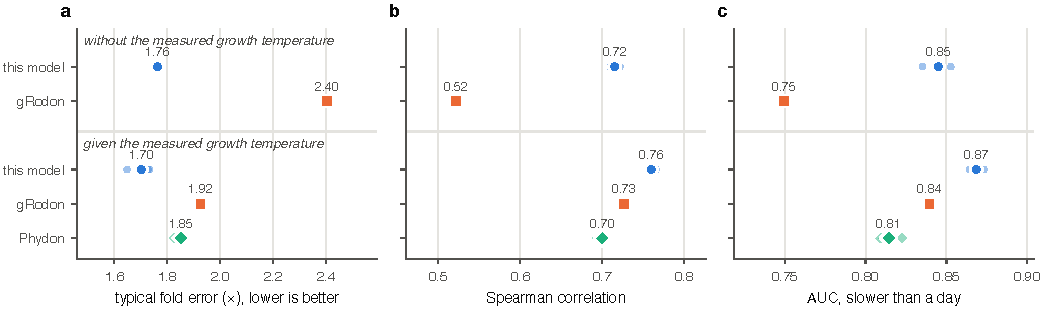
\includegraphics[width=\textwidth]{fig3_released_tools}
\caption{The released gRodon and Phydon against this model on the same \RelN genomes, genes and species-held-out folds
(\RelNSeeds seeds; small marks are seeds, large marks their mean). Both released tools take the measured growth
temperature, which an uncultured genome does not come with; this model is shown without it and with it added as an input.
(a) Typical fold error. (b) Spearman correlation. (c) Area under the curve for a doubling time above one day.}
\label{fig:released}
\end{figure}

\subsection{Ablations at each level}
Table~\ref{tab:ablationsfull} gives the absolute values behind the ablation table of the main text, and the family level,
which the main text leaves out.

\begin{table}[ht]\centering\small
\caption{Every ablation at each held-out level, mean (standard deviation) over 10 seeds, with the deployed settings and each genome entered once. The ablation table of the main text gives the paired changes at the species and order levels.}\label{tab:ablationsfull}
\begin{tabular}{lccc}
\toprule
& Typical error ($\times$) & Spearman & AUC, slow \\
\midrule
\multicolumn{4}{l}{\textit{Species held out}} \\
\quad final model & 1.819 (0.013) & 0.740 (0.005) & 0.838 (0.005) \\
\quad without gRodon statistics & 1.929 (0.024) & 0.697 (0.005) & 0.828 (0.005) \\
\quad without lifestyle genes & 1.824 (0.016) & 0.738 (0.005) & 0.838 (0.005) \\
\quad without any gene features & 2.092 (0.029) & 0.662 (0.004) & 0.806 (0.007) \\
\quad without 16S & 1.817 (0.018) & 0.742 (0.006) & 0.839 (0.005) \\
\quad without GTDB phylogeny & 1.844 (0.029) & 0.732 (0.005) & 0.840 (0.005) \\
\quad without the added species & 1.859 (0.031) & 0.732 (0.007) & 0.836 (0.005) \\
\quad with energy-metabolism genes & 1.820 (0.014) & 0.740 (0.005) & 0.839 (0.005) \\
\quad with predicted growth temperature & 1.804 (0.026) & 0.739 (0.005) & 0.839 (0.005) \\
\addlinespace
\multicolumn{4}{l}{\textit{Family held out}} \\
\quad final model & 2.049 (0.035) & 0.675 (0.010) & 0.808 (0.006) \\
\quad without gRodon statistics & 2.269 (0.066) & 0.600 (0.016) & 0.770 (0.013) \\
\quad without lifestyle genes & 2.047 (0.038) & 0.673 (0.011) & 0.808 (0.007) \\
\quad without any gene features & 2.515 (0.075) & 0.510 (0.024) & 0.741 (0.018) \\
\quad without 16S & 2.029 (0.021) & 0.679 (0.008) & 0.802 (0.008) \\
\quad without GTDB phylogeny & 2.038 (0.042) & 0.673 (0.011) & 0.812 (0.007) \\
\quad without the added species & 2.080 (0.049) & 0.667 (0.008) & 0.807 (0.007) \\
\quad with energy-metabolism genes & 2.055 (0.033) & 0.672 (0.009) & 0.809 (0.005) \\
\quad with predicted growth temperature & 2.047 (0.046) & 0.675 (0.010) & 0.810 (0.006) \\
\addlinespace
\multicolumn{4}{l}{\textit{Order held out}} \\
\quad final model & 2.093 (0.028) & 0.654 (0.010) & 0.803 (0.009) \\
\quad without gRodon statistics & 2.388 (0.051) & 0.574 (0.014) & 0.759 (0.012) \\
\quad without lifestyle genes & 2.074 (0.032) & 0.660 (0.009) & 0.805 (0.008) \\
\quad without any gene features & 2.644 (0.049) & 0.460 (0.017) & 0.727 (0.015) \\
\quad without 16S & 2.093 (0.032) & 0.654 (0.012) & 0.793 (0.010) \\
\quad without GTDB phylogeny & 2.070 (0.026) & 0.657 (0.008) & 0.809 (0.009) \\
\quad without the added species & 2.133 (0.025) & 0.650 (0.012) & 0.797 (0.008) \\
\quad with energy-metabolism genes & 2.107 (0.036) & 0.654 (0.010) & 0.802 (0.008) \\
\quad with predicted growth temperature & 2.078 (0.028) & 0.659 (0.012) & 0.805 (0.010) \\
\bottomrule
\end{tabular}
\end{table}


\subsection{A learned-representation baseline}
Table~\ref{tab:esm} compares protein language-model embeddings with the genome features on the folds of the headline
(Methods of the main text).

\begin{table}[ht]\centering\small\setlength{\tabcolsep}{4pt}
\caption{A learned-representation baseline: ESM-2 (35M) protein embeddings of 742 genomes (mean of all ribosomal proteins and of 100 other proteins per genome) against the genome features, on the folds of the headline, deployed settings, each genome once, mean of 3 seeds. Error: typical fold error of the doubling time at the growth temperature; $\rho$: Spearman correlation.}\label{tab:esm}
\begin{tabular}{lcccccccc}
\toprule
& \multicolumn{2}{c}{same genus} & \multicolumn{2}{c}{new genus} & \multicolumn{2}{c}{new family} & \multicolumn{2}{c}{new order} \\
\cmidrule(lr){2-3} \cmidrule(lr){4-5} \cmidrule(lr){6-7} \cmidrule(lr){8-9}
& Error & $\rho$ & Error & $\rho$ & Error & $\rho$ & Error & $\rho$ \\
\midrule
genome features & 1.82 & 0.74 & 1.96 & 0.71 & 2.07 & 0.67 & 2.08 & 0.67 \\
ESM-2, ridge probe & 1.86 & 0.75 & 1.90 & 0.73 & 2.00 & 0.69 & 2.02 & 0.68 \\
ESM-2, trees on 64 PCs & 2.03 & 0.71 & 2.11 & 0.67 & 2.19 & 0.62 & 2.23 & 0.61 \\
genome features + 32 ESM-2 PCs & 1.78 & 0.76 & 1.91 & 0.74 & 2.03 & 0.70 & 2.05 & 0.70 \\
\bottomrule
\end{tabular}
\end{table}


\subsection{Species from other sources}
As a check that does not depend on how the folds are drawn, the final model was trained on gRodon's growth table alone and
tested on every labeled species of the other sources whose species group is not in that table (Table~\ref{tab:independent}).
The typical error over the \IndepN bacterial species is \IndepErr-fold. The archaeal rows show what happens with no archaea
in training and are not a fair test of the deployed model, which is trained on archaea.

\begin{table}[ht]\centering\small
\caption{Species that are not in gRodon's growth table, predicted by the final model trained on that table alone (294 genomes, no archaea), averaged over five seeds. Error is the typical fold error; $\rho$ the Spearman correlation. The training set is less than half of the full one, so these errors are higher than those of the deployed model; the test shows how the model carries to species from other sources.}\label{tab:independent}
\begin{tabular}{lccccc}
\toprule
& & \multicolumn{2}{c}{At the growth temperature} & \multicolumn{2}{c}{At 20 \textdegree C} \\
\cmidrule(lr){3-4} \cmidrule(lr){5-6}
& Species & Error & $\rho$ & Error & $\rho$ \\
\midrule
\multicolumn{6}{l}{\textit{Bacteria, by closest relative in gRodon's growth table}} \\
\quad same genus & 44 & 1.85 & 0.31 & 1.58 & 0.81 \\
\quad same family, new genus & 76 & 1.82 & 0.66 & 1.91 & 0.75 \\
\quad same order, new family & 68 & 1.91 & 0.51 & 1.78 & 0.83 \\
\quad new order & 106 & 2.65 & 0.39 & 2.09 & 0.63 \\
\quad all bacteria & 294 & 2.09 & 0.61 & 1.87 & 0.78 \\
Archaea (none in training) & 150 & 2.46 & 0.57 & 2.54 & 0.43 \\
\bottomrule
\end{tabular}
\end{table}


\subsection{Metagenome-assembled genomes by species}
\begin{longtable}{p{6.2cm}cccc}
\caption{Doubling time at the growth temperature predicted from metagenome-assembled genomes (MAGs, median over the species' MAGs) and from the isolate genome, with the species held out of training, for the 47 species with a measured value and at least one GEM genome; 717 MAGs in all. Both predictions use the model without 16S, which every MAG can be given.}\label{tab:mags}\\
\toprule
Species & MAGs & Measured (h) & Isolate (h) & MAGs (h) \\
\midrule
\endfirsthead
\caption[]{(continued)}\\
\toprule
Species & MAGs & Measured (h) & Isolate (h) & MAGs (h) \\
\midrule
\endhead
\textit{Acinetobacter baumannii} & 7 & 0.73 & 1.22 & 1.17 \\
\textit{Aeromonas hydrophila} & 1 & 0.33 & 0.67 & 0.78 \\
\textit{Allisonella histaminiformans} & 1 & 1.83 & 0.70 & 0.96 \\
\textit{Bacillus licheniformis} & 1 & 0.58 & 0.70 & 1.10 \\
\textit{Bacillus subtilis} & 4 & 0.24 & 0.68 & 1.02 \\
\textit{Bacteroides fragilis} & 19 & 0.44 & 1.97 & 1.53 \\
\textit{Bacteroides thetaiotaomicron} & 11 & 1.47 & 2.94 & 1.32 \\
\textit{Bifidobacterium longum} & 59 & 1.51 & 1.80 & 1.94 \\
\textit{Caldicellulosiruptor obsidiansis} & 1 & 0.92 & 2.57 & 3.34 \\
\textit{Caldicellulosiruptor owensensis} & 2 & 5.41 & 2.00 & 1.93 \\
\textit{Caldilinea aerophila} & 2 & 5.00 & 14.24 & 13.81 \\
\textit{Chloroflexus aurantiacus} & 3 & 2.31 & 12.19 & 12.03 \\
\textit{Corynebacterium pseudodiphtheriticum} & 1 & 0.62 & 2.80 & 2.73 \\
\textit{Cronobacter sakazakii} & 1 & 0.23 & 0.39 & 0.51 \\
\textit{Cutibacterium acnes} & 127 & 5.10 & 2.82 & 2.81 \\
\textit{Dehalococcoides mccartyi\_B} & 2 & 19.20 & 10.16 & 9.30 \\
\textit{Dictyoglomus thermophilum} & 3 & 2.47 & 1.51 & 1.44 \\
\textit{Enterococcus faecalis} & 50 & 0.38 & 1.13 & 0.71 \\
\textit{Escherichia coli} & 178 & 0.18 & 0.64 & 0.64 \\
\textit{Fusobacterium nucleatum} & 2 & 0.47 & 0.86 & 0.93 \\
\textit{Isosphaera pallida} & 1 & 17.35 & 11.71 & 12.01 \\
\textit{Klebsiella pneumoniae} & 29 & 0.34 & 0.39 & 0.40 \\
\textit{Lactobacillus acidophilus} & 1 & 1.10 & 0.67 & 0.75 \\
\textit{Lactococcus lactis} & 14 & 0.39 & 0.50 & 0.67 \\
\textit{Leifsonia xyli\_A} & 1 & 5.50 & 2.28 & 1.39 \\
\textit{Meiothermus ruber} & 1 & 1.67 & 2.07 & 2.01 \\
\textit{Mesotoga prima} & 3 & 16.50 & 3.45 & 4.17 \\
\textit{Nitrosomonas europaea} & 5 & 5.50 & 6.16 & 6.81 \\
\textit{Persephonella marina} & 7 & 3.35 & 1.61 & 1.51 \\
\textit{Porphyromonas gingivalis} & 11 & 2.56 & 6.57 & 6.34 \\
\textit{Pseudomonas aeruginosa} & 5 & 0.33 & 0.52 & 0.68 \\
\textit{Psychrobacter cryohalolentis} & 2 & 2.62 & 2.23 & 2.22 \\
\textit{Rhodopirellula baltica} & 1 & 10.00 & 12.71 & 12.29 \\
\textit{Sinorhizobium meliloti} & 1 & 1.50 & 2.08 & 1.47 \\
\textit{Staphylococcus aureus} & 1 & 0.45 & 0.46 & 0.62 \\
\textit{Staphylococcus epidermidis} & 22 & 0.33 & 0.54 & 0.65 \\
\textit{Streptococcus mutans} & 2 & 1.10 & 0.79 & 0.79 \\
\textit{Streptococcus thermophilus} & 9 & 0.29 & 0.43 & 0.47 \\
\textit{Syntrophobacter fumaroxidans} & 1 & 98.00 & 7.46 & 7.72 \\
\textit{Syntrophus aciditrophicus} & 1 & 27.00 & 3.65 & 3.68 \\
\textit{Thermobaculum terrenum} & 6 & 4.09 & 3.78 & 3.36 \\
\textit{Thermodesulfobacterium commune} & 1 & 2.31 & 1.98 & 1.77 \\
\textit{Thermus aquaticus} & 4 & 0.69 & 0.76 & 0.80 \\
\textit{Thermus brockianus} & 1 & 1.07 & 0.84 & 0.85 \\
\textit{Thermus thermophilus} & 110 & 0.29 & 0.93 & 0.90 \\
\textit{Vibrio alginolyticus} & 1 & 0.25 & 0.46 & 0.46 \\
\textit{Vibrio cholerae} & 1 & 0.35 & 0.43 & 0.47 \\
\bottomrule
\end{longtable}


\subsection{The low-energy test, every input}
Table~\ref{tab:pgls} gives every input of the low-energy test with the three checks described in the Methods. No input that
describes how an organism makes energy reaches an adjusted $p<0.05$ in the main analysis or in any of these three checks. With $\lambda$
fixed at 1, complex I and the number of terminal oxidases go with faster growth; with only the groups placed at their own
GTDB species, catalase does. Regulator density goes with faster growth in the main analysis and in two of the three checks,
but not with $\lambda$ fixed at 1.

{\small\setlength{\tabcolsep}{3pt}
\begin{longtable}{p{4.6cm}rrlrrrrr}
\caption{The low-energy test, every input, 592 species groups. Effects are fold changes in doubling time for carrying the gene, per standard deviation of a count or density, or per doubling of genome size, with growth temperature and domain as covariates. With: groups carrying the gene (presence inputs). Across: without control for relatedness. PGLS: phylogenetic generalized least squares with Pagel's $\lambda$ estimated; $p_{\mathrm{adj}}$ is Benjamini-Hochberg adjusted over the inputs. Families: of the families with both carriers and non-carriers, those in which the median carrier is slower. The last three columns give the adjusted PGLS $p$ with $\lambda$ fixed at 1, with only the groups placed at their own GTDB species, and without the eight literature strains.}\label{tab:pgls}\\
\toprule
Input & With & Across & PGLS (95\% CI) & $p_{\mathrm{adj}}$ & Families & $\lambda=1$ & Own sp. & No lit. \\
\midrule
\endfirsthead
\caption[]{(continued)}\\
\toprule
Input & With & Across & PGLS (95\% CI) & $p_{\mathrm{adj}}$ & Families & $\lambda=1$ & Own sp. & No lit. \\
\midrule
\endhead
aerobic respiration (terminal oxidase) & 393 & 1.14 & 1.01 (0.70--1.45) & 0.992 & 4/8 & 0.601 & 0.904 & 0.993 \\
complex I & 502 & 1.58 & 0.97 (0.72--1.31) & 0.992 & 6/18 & $<$0.001 & 0.886 & 0.993 \\
methanogenesis & 39 & 0.74 & 0.75 (0.27--2.06) & 0.913 & -- & 0.962 & 0.846 & 0.971 \\
sulfate reduction & 24 & 2.84 & 1.33 (0.64--2.78) & 0.852 & 0/2 & 0.962 & 0.846 & 0.754 \\
nitrogen fixation & 128 & 1.52 & 1.18 (0.93--1.50) & 0.595 & 13/26 & 0.385 & 0.846 & 0.435 \\
RuBisCO (carbon fixation) & 172 & 1.21 & 1.15 (0.90--1.46) & 0.700 & 12/26 & 0.332 & 0.846 & 0.697 \\
ammonia or methane oxidation & 7 & 3.76 & 1.49 (0.47--4.77) & 0.901 & -- & 0.962 & 0.846 & 0.993 \\
phototrophy & 31 & 2.51 & 0.92 (0.52--1.65) & 0.992 & 3/6 & 0.962 & 0.904 & 0.993 \\
flagellar motility & 320 & 0.90 & 1.07 (0.80--1.43) & 0.913 & 4/17 & 0.962 & 0.904 & 0.971 \\
catalase & 184 & 0.48 & 0.74 (0.59--0.92) & 0.094 & 16/37 & 0.601 & 0.038 & 0.074 \\
nitrate respiration & 135 & 0.51 & 0.94 (0.72--1.21) & 0.913 & 10/23 & 0.962 & 0.846 & 0.971 \\
denitrification (NosZ) & 63 & 0.95 & 1.04 (0.79--1.38) & 0.992 & 10/24 & 0.962 & 0.886 & 0.971 \\
DMSO/TMAO respiration & 62 & 0.88 & 0.99 (0.73--1.34) & 0.992 & 4/13 & 0.339 & 0.904 & 0.993 \\
fumarate respiration (E. coli type) & 46 & 0.56 & 0.88 (0.55--1.40) & 0.913 & 4/7 & 0.810 & 0.904 & 0.971 \\
metal reduction outside the cell & 16 & 0.47 & 0.64 (0.39--1.06) & 0.393 & 3/8 & 0.339 & 0.505 & 0.435 \\
Wood-Ljungdahl pathway & 66 & 1.29 & 1.19 (0.83--1.72) & 0.763 & 3/9 & 0.962 & 0.886 & 0.697 \\
F-type ATP synthase & 442 & 0.68 & 0.62 (0.39--0.99) & 0.340 & 1/7 & 0.601 & 0.251 & 0.321 \\
V/A-type ATP synthase & 203 & 1.17 & 1.21 (0.92--1.60) & 0.595 & 9/18 & 0.719 & 0.792 & 0.511 \\
Na$^+$-NQR & 67 & 0.42 & 0.76 (0.51--1.15) & 0.595 & 5/9 & 0.859 & 0.792 & 0.624 \\
Rnf complex & 241 & 0.76 & 0.96 (0.77--1.18) & 0.943 & 20/34 & 0.589 & 0.904 & 0.993 \\
Na$^+$-pumping decarboxylase & 171 & 1.03 & 1.15 (0.89--1.48) & 0.713 & 9/17 & 0.339 & 0.846 & 0.697 \\
fermentation only & 122 & 1.04 & 0.98 (0.68--1.39) & 0.992 & 7/11 & 0.962 & 0.846 & 0.993 \\
transporter density (per SD) & -- & 0.83 & 0.88 (0.77--1.00) & 0.340 & -- & 0.478 & 0.085 & 0.435 \\
regulator density (per SD) & -- & 0.78 & 0.80 (0.70--0.92) & 0.042 & -- & 0.408 & 0.018 & 0.049 \\
number of terminal oxidases (per SD) & -- & 0.93 & 0.92 (0.81--1.05) & 0.595 & -- & 0.022 & 0.846 & 0.435 \\
number of hydrogenases (per SD) & -- & 1.20 & 1.13 (1.00--1.27) & 0.340 & -- & 0.962 & 0.792 & 0.321 \\
number of electron acceptor classes (per SD) & -- & 0.92 & 0.99 (0.87--1.13) & 0.992 & -- & 0.601 & 0.904 & 0.993 \\
number of sodium pumps (per SD) & -- & 0.87 & 1.00 (0.88--1.13) & 0.992 & -- & 0.962 & 0.904 & 0.993 \\
genome size (per doubling) & -- & 0.90 & 0.91 (0.75--1.12) & 0.814 & -- & 0.332 & 0.846 & 0.697 \\
\bottomrule
\end{longtable}}


\section{Data, code and reproduction}

\subsection{What is released}
The repository and its Zenodo archive hold the code, the curated labels (\texttt{data/curated}), the prediction table for
the GEM genomes (\texttt{release/gem\_growth\_predictions.csv}, Table~\ref{tab:columns}), and the derived tables and result
files of \texttt{data/processed} that the paper is built from. With the archive unpacked in the repository, the numbers,
tables and figures of the paper are rebuilt from the result files by \texttt{make} in \texttt{paper/}, and every model is
retrained and evaluated from the derived tables without downloading genomes. We checked this by unpacking the archive in
an empty folder: every number and table rebuilt from it was identical to those printed here, and retraining the models from it gave the
same GEM predictions.

Each prediction in the table carries the error and the 80\% range measured for its model and novelty level, for the
doubling time at the growth temperature, the doubling time at \TRefC\,\textdegree C and the growth temperature. The
novelty level is computed from the GTDB names in the GEM metadata, which come from an older GTDB release than the training
data, so it is a worst case.

\begin{longtable}{p{5.9cm}p{9.9cm}}
\caption{Columns of the released prediction table for the GEM genomes, \texttt{gem\_growth\_predictions.csv}.}\label{tab:columns}\\
\toprule
Column & Meaning \\
\midrule
\endfirsthead
\caption[]{(continued)}\\
\toprule
Column & Meaning \\
\midrule
\endhead
\texttt{genome\_id} & GEM genome identifier (Nayfach et al. 2021) \\
\texttt{gtdb\_taxonomy} & GTDB taxonomy from the GEM metadata (an older GTDB release than the training data, so the novelty level is a worst case) \\
\texttt{nearest\_labeled\_relative} & closest rank shared with a labeled training species: same genus, same family, new genus, same order, new family, or new order \\
\texttt{doubling\_time\_h} & predicted maximal doubling time at the predicted growth temperature, hours \\
\texttt{doubling\_time\_low\_h} & lower end of the 80\% range, hours \\
\texttt{doubling\_time\_high\_h} & upper end of the 80\% range, hours \\
\texttt{doubling\_time\_fold\_error} & typical fold error at this novelty level (median of measured/predicted or its inverse) \\
\texttt{doubling\_time\_20C\_h} & predicted doubling time standardized to 20 C, hours \\
\texttt{doubling\_time\_20C\_low\_h} & lower end of the 80\% range, hours \\
\texttt{doubling\_time\_20C\_high\_h} & upper end of the 80\% range, hours \\
\texttt{doubling\_time\_20C\_fold\_error} & typical fold error at this novelty level \\
\texttt{growth\_temp\_c} & predicted optimal growth temperature, C \\
\texttt{growth\_temp\_low\_c} & lower end of the 80\% range, C \\
\texttt{growth\_temp\_high\_c} & upper end of the 80\% range, C \\
\texttt{growth\_temp\_error\_c} & mean absolute error at this novelty level, C \\
\texttt{slower\_than\_a\_day} & predicted doubling time above 24 hours \\
\texttt{prob\_slower\_than\_a\_day} & calibrated probability that the doubling time is above 24 hours (useful for ranking; the model rarely predicts above a day for a new lineage) \\
\texttt{model\_used} & inputs available for this genome, and so the model used \\
\texttt{domain} & bacteria or archaea \\
\texttt{phylogeny\_rank\_used} & GTDB rank at which the genome was placed for the phylogeny input; empty when the genome could not be placed \\
\texttt{completeness} & CheckM completeness, \% (GEM metadata) \\
\texttt{contamination} & CheckM contamination, \% (GEM metadata) \\
\texttt{ecosystem\_category} & GEM metadata \\
\texttt{ecosystem\_type} & GEM metadata \\
\texttt{habitat} & GEM metadata \\
\bottomrule
\end{longtable}


\subsection{Reproducing the results}
From an empty checkout, \texttt{make paper} downloads every input at the version used here, runs the whole chain and
builds the PDFs; it takes about a day on ten cores, most of it in the gene predictions for the GEM genomes and in the nested
evaluation. \texttt{make verify-inputs} checks the downloaded files against their SHA-256 checksums
(\texttt{data/input\_checksums.tsv}), and \texttt{REPRODUCE.md} in the repository lists the software versions and the
pinned data sources. Table~\ref{tab:reproduce} gives the
step behind each result. Every number in the text is a macro in \texttt{paper/numbers.tex}, written by
\texttt{paper/scripts/make\_numbers.py}, and \texttt{paper/numbers\_sources.csv} gives the file each comes from.

\begin{table}[ht]\centering\footnotesize
\caption{The step behind each result. Make targets are run from the repository root; scripts are in
\texttt{scripts/accuracy} unless a folder is given; outputs are in \texttt{data/processed} unless a folder is given.}\label{tab:reproduce}
\begin{tabular}{>{\raggedright}p{3.4cm}>{\raggedright}p{2.7cm}>{\raggedright\arraybackslash}p{9.6cm}}
\toprule
Result & Make target & Script $\to$ output \\
\midrule
Training data and labels & \texttt{predict-all} & \texttt{src/.../deploy\_features.py} \newline $\to$ read at run time \\
Label audit and its controls & \texttt{label-check, paper-results} & \texttt{screen\_label\_sources.py, audit\_controls.py} \newline $\to$ \texttt{label\_sources\_studies.csv, audit\_controls.csv} \\
Accuracy by novelty & \texttt{paper-results} & \texttt{evaluate\_paper\_headline.py} \newline $\to$ \texttt{paper\_headline\_accuracy.csv, paper\_headline\_predictions.csv} \\
Deployed errors and ranges & \texttt{accuracy-table} & \texttt{evaluate\_final\_model.py} \newline $\to$ \texttt{final\_accuracy\_by\_tier.csv} \\
Released gRodon and Phydon & \texttt{released-tools, paper-results} & \texttt{compare\_released\_tools.py, scripts/r/*.R} \newline $\to$ \texttt{released\_tools\_comparison\_nested.csv} \\
Ablations and learner & \texttt{paper-results} & \texttt{evaluate\_ablations.py, evaluate\_tuning.py} \newline $\to$ \texttt{ablation\_evaluation.csv, tuning\_evaluation.csv} \\
16S source & \texttt{paper-results} & \texttt{evaluate\_16s\_source.py} \newline $\to$ \texttt{16s\_source\_evaluation.csv} \\
Baselines, intervals, shuffled labels, paired tests & \texttt{paper-results} & \texttt{pressure\_tests.py} \newline $\to$ \texttt{pressure\_tests.csv} \\
Metagenome-assembled genomes & \texttt{paper-results} & \texttt{validate\_on\_gem\_mags.py} \newline $\to$ \texttt{mag\_validation.csv} \\
Species from other sources & \texttt{paper-results} & \texttt{evaluate\_independent\_species.py} \newline $\to$ \texttt{independent\_test.csv} \\
Low-energy test and syntrophy & \texttt{lifestyle-test} & \texttt{test\_lifestyle\_phylogenetic.py, check\_lifestyle\_phylogenetic.py, evaluate\_syntrophy\_marker.py} \newline $\to$ \texttt{lifestyle\_phylogenetic\_test.csv, lifestyle\_phylogenetic\_checks.txt, syntrophy\_marker.csv} \\
GEM predictions & \texttt{predict} & \texttt{scripts/pipeline/predict\_gem\_genomes\_gbm.py, scripts/pipeline/export\_hq\_table.py} \newline $\to$ \texttt{hq\_predictions\_gbm.csv, release/gem\_growth\_predictions.csv} \\
Numbers, tables, figures & \texttt{make} in \texttt{paper/} & \texttt{paper/scripts/*.py} \newline $\to$ \texttt{paper/numbers.tex}, tables, figures \\
\bottomrule
\end{tabular}
\end{table}

\bibliographystyle{unsrtnat}
\bibliography{refs}
\end{document}
